\documentclass{article}
\usepackage{style}

% Additional packages
\usepackage{subfig,float}
%\captionsetup[subfloat]{farskip=-1mm,captionskip=-1mm}
\newcommand{\twa}{0.45\textwidth}
\newcommand{\twb}{0.3333333333\textwidth}
\usepackage{tabularx}
%\newcolumntype{C}[1]{>{\centering\arraybackslash$}p{#1}<{$}}
\setlength{\arrayrulewidth}{1.0pt}

% Define colors
\usepackage{color}
\definecolor{orange}{rgb}{1,0.5,0}
\definecolor{amethyst}{rgb}{0.6,0.4,0.8}
\definecolor{aureolin}{rgb}{0.99,0.93,0.0}
\definecolor{awesome}{rgb}{1.0,0.13,0.32}
\definecolor{ao-green}{rgb}{0.0, 0.5, 0.0}
\definecolor{MSBlue}{rgb}{.204,.353,.541}

% Define commands for communication between us
\newcommand{\ferran}[1]{\textcolor{green}{#1}}
\newcommand{\javier}[1]{\textcolor{blue}{#1}}
\newcommand{\lluis}[1]{\textcolor{orange}{#1}}
\newcommand{\chat}[1]{\textcolor{amethyst}{#1}}
\newcommand{\review}[1]{\textcolor{red}{#1}}

%commands to manage sections, figures and acronyms
\usepackage{doi}
%\usepackage{tikz}
%\usetikzlibrary {positioning,intersections,fit,shapes.geometric}
%\newcommand{\fig}[1]{Figure~\ref{fig:#1}}
%\newcommand{\sect}[1]{Section~\ref{sec:#1}}
\usepackage{acronym}
\acrodef{hpc}[HPC]{high performance computing}
\acrodef{cpu}[CPU]{central process unit}
\acrodef{gpu}[GPU]{graphics processing unit}
\acrodef{dns}[DNS]{direct numerical simulation}
\acrodef{mhd}[MHD]{magneto-hydro-dinamics}
\acrodef{upo}[UPO]{unstable periodic orbit}
\acrodef{pod}[POD]{proper orthogonal decomposition}
\acrodef{dmd}[DMD]{dynamic mode decomposition}
\acrodef{sindy}[SINDy]{sparse identification of nonlinear dynamical systems}
\acrodef{bvae}[$\beta$-VAE]{beta-variational autoencoders}
\acrodef{res}[RES]{Red Española de Supercomputación}
\acrodef{prace}[PRACE]{Partnership for Advanced Computing in Europe}
\acrodef{bsc}[BSC]{Barcelona Supercomputing Center}
\acrodef{upc}[UPC]{Universitat Polit\`ecnica de Catalunya $\cdot$ BarcelonaTech}


\usepackage{pgfplots}
\usepackage{graphicx}
\usepackage{fancyhdr}
\pagestyle{fancy}
%\usepackage{xcolor}
\usepackage[dvipsnames]{xcolor}
\usepackage{lipsum}
\setlength\headheight{26pt} %%
\usepackage{hyperref}
\usepackage[final]{pdfpages}
\usepackage{stix}
\usepackage{float}
\usepackage{caption}
\newcounter{includepdfpage}
\usepackage{tabularx}
\usetikzlibrary {arrows.meta} 
\usetikzlibrary{decorations.markings}
\usepgfplotslibrary{colormaps}
\usepackage[titles]{tocloft}
\setlength{\cftbeforechapskip}{15pt}
%\pgfplotsset{width=7cm,compat=newest,axis line style={draw=none},ticks=none}

%\lhead{\includegraphics[width=0.2\textwidth]{nyush-logo.pdf}}

%\fancypagestyle{firstpage}{%
%  \rhead{\Large HAP-Calafell}
%  \lhead{
\includegraphics[width=5cm]{logo-upc}}
%}

\fancypagestyle{firststyle}
{
   \fancyhf{}
   \fancyhead[L]{
\includegraphics[width=5cm]{logo-upc}}
   \fancyhead[R]{\Large HAP-Calafell}
}

\pagestyle{fancy}
\fancyhf{}
\fancyhead[L]{
\includegraphics[width=5cm]{logo-upc}}
\fancyhead[R]{\Large HAP-Calafell}
\fancyfoot[R]{Page \thepage}

%%%% PROJECT TITLE
\title{{\bf Historial Acadèmic i Professional / \\ Academic and Professional Record}}
\date{}
\author{\Large Joan Calafell Sandiumenge}

\begin{document}

\maketitle


\thispagestyle{firststyle}

\vspace{1.0cm}

\begin{tabular}{ l l }
\hline \\
 Site Code:          & 71025761-71025762  \\ 
 Position Reference: & LE-27-28/729 \\
 Unit of assignment: & 729- Fluid Mechanics Department  \\  
 Field of Knowledge: & Industrial Engineering \\
 Area of Knowledge:  & Fluid Mechanics \\   
 Linked Unit:        & Escola d’Enginyeria Barcelona Est (EEBE)\\
  $\ $               & $\quad $$\quad $$\quad $$\quad $$\quad $$\quad $$\quad $$\quad $$\quad $$\quad $$\quad $$\quad $$\quad $$\quad $$\quad $$\quad $$\quad $$\quad $$\quad $$\quad $$\quad $$\quad $$\quad $$\quad $$\quad $$\quad $$\quad $$\quad $$\quad $$\quad $$\quad $$\quad $$\quad $$\quad $$\quad $$\quad $$\quad $$\quad $\\
 \hline
\end{tabular}

\newpage

\tableofcontents

\newpage

\section{Academic and Professional Record}
\subsection{Personal Data}

\vspace{0.5cm}

\begin{tabular}{ l l }
 {\bf Name:}               & Joan Calafell Sandiumenge  \\ 
 {\bf ID Number:}          & 44019853S \\
 {\bf Nationality:}        & Spanish  \\  
 {\bf Date of Birth:}      & 14/06/1978 \\
 {\bf Address:}            & Guifré 8 3er 1a 08001 Barcelona \\   
 {\bf Phone:}              & +34 669 14 36 49\\
 {\bf E-mail:}             & joan.calafell@upc.edu\\
\end{tabular}

\vspace{0.5cm}

\subsection{Academic Qualifications}

\begin{itemize}
\item {\bf 2021:} Postgraduate Degree in Deep Learning. Universitat Politècnica de Catalunya. Final Mark: 8.5 out of 10. \hyperlink{postgrau-DL.1}{(see document)}
\item {\bf 2019:} Ph.D. in Computational Science applied to Fluid Mechanics. Universitat Politècnica de Catalunya. Final Mark: Excellent Cum Laude {\bf with International Mention}. 
\hyperlink{doctorat.1}{(see document)}
\item {\bf 2011:} Master in Energy (60 ECTS including Master thesis). Universitat Politècnica de Catalunya. Final Mark: 9.90 out of 10. \hyperlink{master-E.1}{(see document)}
\item {\bf 2003:} Master in Industrial Engineering (Enginyeria Superior Industrial). Universitat Politècnica de Catalunya. 2003. Final Mark: 6.16 out of 10.  \hyperlink{carrera-EI.1}{(see document)}
\end{itemize}

\subsection{Academic and Professional Positions}

\begin{itemize}
\item {\bf Sep 2022-present:} Assistant professor (ATP) at {\bf Universitat Politècnica de Catalunya}. Professor of the core subjects of Thermal Engines  (Màquines Tèrmiques, 240EI021, 4.5 ECTS) and Heat Transfer (Termotècnia, 240171, 6 ECTS), theoretical and numerical laboratory sessions.

\item {\bf Nov 2019-present:} Recognized Researcher (R2) at {\bf Barcelona Supercomputing Center}. 

\item  {\bf Apr 2017-Jul 2017:} Research visitor at the {\bf Aerospace Computational Design Laboratory at the Massachusetts Institute of Technology}. \hyperlink{mit.1}{(see ref. letter)}

\item {\bf Jan 2017-Oct 2019:} Ph.D. student at {\bf Centre Tecnològic de Transferència de Calor of the Universitat Politècnica de Catalunya.} 

\item  {\bf Dec 2011-Jan 2017:} Industrial Ph.D. student, software and project developer at Termo Fluids S.L. \hyperlink{termofluids.1}{(see ref. letter)}

\item  {\bf Mar 2008-Jul 2010:} R\&D Engineer at C\&G Carandini. \hyperlink{carandini.1}{(see ref. letter)}

\item  {\bf Mar 2005-Mar 2008:} R\&D Engineer at {\bf Nissan Motor Ibérica}. \hyperlink{nissan.1}{(see ref. letter)}

\item  {\bf Jul 2001-Jul 2004:} Lecturer of Mathematics, Physics, Mechanics, Electro Technology, and Technology at Acadèmica Blancafort. 

\end{itemize}


\subsection{Acreditations}
\begin{itemize}
\item Acreditación Ayudante Doctor ANECA. {\bf Issuing date: 18/05/2023 (Three days after the submission deadline)} \hyperlink{acreditacio.1}{(see document)}
\end{itemize}

\subsection{Competitive Grants}

\begin{itemize}
\item {\bf Dec 2011-Nov 2014:} Talent Empresa ({\it TEM-DGR 2010}). Industrial Ph.D. Grant of AGAUR. Total funding: 43.890,00€. \hyperlink{agaur.1}{(see document)}
\end{itemize}

\subsection{Seminars and training received}

\begin{itemize}
\item {\bf Dec 2022:} Public Speech Training. Entity: Barcelona Supercomputing Center. Number of hours: 12. 
\item {\bf Oct 2021:} Project Management. Entity: Barcelona Supercomputing Center. Number of hours: 12. 
\item {\bf Oct 2020:} Parallel Programming Workshop. Entity: PRACE and Barcelona Supercomputing Center. Number of hours: 16. 
\item {\bf May 2018:} Mathematical Foundations of Computational Fluid Dynamics (MathCFD). Entity: Centre Tecnològic de Transferència de Calor. Number of hours: 22. 
\end{itemize}

\newpage

\section{Teaching Record}
\subsection{Undergraduate courses taught}
\begin{itemize}
\item {\bf Feb 2023-present:} Heat Transfer theory (Termotècnia, 240171). Credits: 6 ECTS. Core subject of the Industrial Engineering Bachelor Degree (GETI) at the "Escola Tècnica Superior d’Enginyeria Industrial de Barcelona" (ETSEIB). 
\end{itemize}

\subsection{Master's courses taught}
\begin{itemize}
\item {\bf Sep 2022-present:} Thermal Machines theory (Màquines Tèrmiques, 240EI021). Credits: 4.5 ECTS. Core subject of the Master in Industrial Engineering (MUEI) at ETSEIB.
\end{itemize}

\subsection{University preparatory courses:}
\begin{itemize}
\item {\bf June 2001-Jul 2004:}  Lecturer of Mathematics, Physics, Technology, Mechanics, and Electrical Technology at university access level. Acadèmia Blancafort (Barcelona).
\end{itemize}
\subsection{Bachelor thesis directed and advised}

\begin{itemize}
\item {\bf 2023 spring term (ongoing):} Title: Autoencoders for fluid flow data compression. Student: Joan Julián Vergés. Contribution: co-director. \hyperlink{tfg.1}{(see ref. letter)}
\item {\bf 2022 spring term:} Title: Discovering new scaling laws in turbulent boundary layers via multi-expression programming. Student: Irene Simó Muñoz. Contribution: advisor. \hyperlink{tfg.1}{(see ref. letter)}
\end{itemize}

\subsection{Ph.D. thesis advised}

\begin{itemize}
\item {\bf 2019-present:} Title: Machine Learning-based Wall Modeling Methods for Large-Eddy Simulation. Student: Sarath Radhakrishnan. Contribution: advisor \hyperlink{tesis.1}{(see ref. letter)}
\end{itemize}

\subsection{Ph.D. research plan comittees}

\begin{itemize}
\item {\bf 2022 fall term:} Title: Shock-induced laminar-to-turbulent transition in supersonic hydrogen flows. Student: Ahmed Mohammed Abdelfattah Abdellatif. \hyperlink{tribunals.1}{(see ref. letter)}
\item {\bf 2022 fall term:} Title: Supercritical miniaturization of wall-bounded turbulence. Student: Marc Ollé Bernades. \hyperlink{tribunals.1}{(see ref. letter)}
\end{itemize}

\subsection{Teaching Material}
\begin{itemize}
\item {\bf 2022-2023 academic year:} I contributed to creating new laboratory sessions for the Thermal Engine Master's subject. 
\end{itemize}

\subsection{Seminars taught}

\begin{itemize}
\item {\bf Feb 2020:} Efficient Wall Modeling for Large Eddy Simulations of General Non-Equilibrium Wall-Bounded Flows. Place: Barcelona Supercomputing Center. Hours: 2.
\end{itemize}

\begin{itemize}
\item {\bf Jan 2014 - Nov 2019:} I took part in several Helicopters (220031,	
Disseny d'Helicòpters i Aeronaus Diverses) and  Wind Energy (820739 - EO - Energía Eólica) subject lectures to teach aerodynamic fundamentals and the use of xfoil code for aerodynamic airfoil simulation.  These subjects are part of the UPC's Aerospace Vehicle Engineering Degree and the Master in Energy, respectively.
\end{itemize}

\subsection{Complementary Teaching Activities}

\begin{itemize}
\item {\bf Feb 2020:} Visit to the MareNostrum Supercomputer at the Barcelona Supercomputing Center facilities for the Thermal Engines students. The concept of massive parallel numerical simulations and the need for HPC were explained.
\item {\bf Jun 2020:} Visit to the MareNostrum Supercomputer at the Barcelona Supercomputing Center facilities for the Heat Transfer and Thermal Engines students. The concept of massive parallel numerical simulations and the need for HPC were explained. 
\end{itemize}

\subsection{Teaching Performance Indicators}

\begin{itemize}
\item UPC Student Satisfaction Survey 2022-23 fall term. First question: 4.88/5.0; Second question: 4.75/5.0 \hyperlink{enquestes.1}{(see document)}. The 2022-23 spring term survey is not available yet.
\end{itemize}

\newpage

\section{Research Record}
\subsection{Research Identificators:}

\vspace{0.5cm}


\begin{tabular}{ l l }
 {\bf Orchid ID:}               & \href{https://orcid.org/0000-0002-2333-7314}{0000-0002-2333-7314}  \\ 
 {\bf Scopus Author ID:}        & 56245196800 \\
 {\bf Google Scholar:}          & \href{https://scholar.google.com/citations?user=wPHQb84AAAAJ&hl=en}{View Google Scholar Profile}  \\  
 {\bf UPC Barcelona Tech:}          & \href{https://futur.upc.edu/JoanCalafellSandiumenge/}{https://futur.upc.edu/JoanCalafellSandiumenge/}  \\ 
\end{tabular}

\vspace{0.5cm}

\subsection{Research Lines and Interests}

My current research lines and interests are focused on the application of state-of-the-art machine learning techniques to solve different challenges in the Computational Fluid Dynamics, Heat, and Mass Transfer areas applied to different technological fields. The main research areas are summarized below, while more details on the specific subtopics are given in the research plan: 

\begin{itemize}
\item Data-Driven non-equilibrium wall models for high-Reynolds and high-Mach number aerodynamic simulations.
\item Computational and fast data-driven urban flow and pollutant transport predictive models. 
\end{itemize}

\subsection{Research Groups}

\begin{itemize}
\item {\bf Dec 2011-Oct 2019:} Centre Tecnològic de Transferència de Calor (CTTC) registered as “Grup de recerca consolidat” by the "Agència de Gestió d'Ajudes Universitaries i d'Investigación" (AGAUR) de la Generalitat de Catalunya (2005SGR00849 / 2009SGR80 / 2014SGR1247). Group Leader: Prof. Assensi Oliva Llena. 

\item {\bf Nov 2019-present:} Large-Scale Computation Fluid Dynamics group, Barcelona Supercomputing Center, registered as “Grup de recerca consolidat” by the "Agència de Gestió d'Ajudes Universitaries i d'Investigació" (AGAUR) de la Generalitat de Catalunya (2021 SGR 00902). Group Leader: Dr. Oriol Lehmkuhl Barba.

\end{itemize}

\subsection{Publications}
\subsubsection{Journal Articles}

\begin{itemize}

\item D. Volkov and J. Calafell. A stochastic approach to reconstruction of faults in elastic half-space. {\it Inverse Problems \& Imaging}, Vol. 13(3) pp. 479-511 (2019) \href{http://dx.doi.org/10.3934/ipi.2019024}{http://dx.doi.org/10.3934/ipi.2019024} ({\bf Scopus Q1})

\item J. Calafell, F.X. Trias, O. Lehmkuhl and A. Oliva. A time-average filtering technique to improve the efficiency of two-layer wall models for large eddy simulation in complex geometries. {\it Computers \& Fluids}, Vol. 188 pp. 49-59 (2019) \href{https://doi.org/10.1016/j.compfluid.2019.03.026}{https://doi.org/10.1016/j.compfluid.2019.03.026} ({\bf Scopus Q1})

\item D.E. Aljure, J. Calafell, A. Baez, A. Oliva. Flow over a realistic car model: Wall modeled large eddy simulations assessment and unsteady effects. {\it Journal of Wind Engineering and Industrial Aerodynamics}, Vol. 174, pp. 225-240 (2018) \href{https://doi.org/10.1016/j.jweia.2017.12.027}{https://doi.org/10.1016/j.jweia.2017.12.027} ({\bf Scopus Q1})

\end{itemize}

\subsubsection{Journal Articles in Preparation}

\begin{itemize}

\item J. Calafell, J. Bustillo, F. Ramírez, S. Gómez, and O. Lehmkuhl. A General Urban Flow Predictor based on Convolutional Neural Networks. To be submitted in {\it Atmospheric Research} (Scopus Q1) in the fourth quarter of 2023. 

\item J. Calafell, J. Bustillo, F. Ramírez, S. Gómez, and O. Lehmkuhl. A high-fidelity dataset for urban flow and pollution dispersion data-driven modeling. To be submitted in {\it Geoscience Data Journal} (Scopus Q1) in the fourth quarter of 2023. 

\item S. Radhakrishnan, J. Calafell, B. Font, A. Miró, and Oriol Lehmkuhl. A non-equilibrium data-driven wall model for complex flows. To be submitted in {\it Physical Review Fluids} (Scopus Q1) in the second half of 2023. 

\end{itemize}

\subsubsection{Conference Articles}

\begin{itemize}

\item S. Radhakrishnan, L. Adu Gyamfi, A. Miró, B. Font, J. Calafell, and Oriol Lehmkuhl. A Data-Driven Wall-Shear Stress Model for LES Using Gradient Boosted Decision Trees. {\it Lecture Notes in Computer Science}, Vol. 12761, pp. 105-121 (2021) 
\href{https://doi.org/10.1007/978-3-030-90539-2_7}{https://doi.org/10.1007/978-3-030-90539-2\_7}

\item D.E. Aljure, J. Calafell, A. Baez, A. Oliva. Flow over a realistic car model: WMLES assessment and turbulent structures.  {\it ERCOFTAC Series}, Vol. 25 pp. 497-503 (2019) \href{https://doi.org/10.1007/978-3-030-04915-7_66}{https://doi.org/10.1007/978-3-030-04915-7\_66}

\item J. Calafell, F.X. Trias, and A. Oliva. An efficient Two-Layer wall model for accurate numerical simulations of aeronautical applications. {\it Proceedings of the 8th European Conference for Aeronautics and Space Sciences. Madrid, Spain, 1-4 July 2019}, (2019) \href{DOI:10.13009/EUCASS2019-694}{DOI:10.13009/EUCASS2019-694}

\item J. Calafell, O. Lehmkuhl, I. Rodríguez, A. Oliva  and C.D. Pérez-Segarra. A dynamic wall model for large eddy simulation on unstructured meshes. Application to wind turbine dedicated airfoils. {\it Proceedings of the International Symposium on Turbulence, Heat and Mass Transfer} (2015) 

\item J. Calafell, O. Lehmkuhl, A. Carmona, C.D. Pérez-Segarra and A. Oliva. A dynamic wall model for large-eddy simulations of wind turbine dedicated airfoils. {\it Journal of Physics: Conference Series}, Vol. 524, (2014) \href{https://doi.org/10.1016/j.jweia.2017.12.027}{https://doi.org/10.1016/j.jweia.2017.12.027}

\item J. Calafell, A. Carmona, O. Lehmkuhl, C.D. Pérez-Segarra and A. Oliva. Dynamic wall modelling for Large-Eddy Simulations. Application to high Reynolds number aerodynamics of complex geometries. {\it 11th World Congress on Computational Mechanics, WCCM 2014, 5th European Conference on Computational Mechanics, ECCM 2014 and 6th European Conference on Computational Fluid Dynamics, ECFD 2014}, pp. 5570-5580, (2014) 

\item J. Calafell, O. Lehmkuhl, I. Rodríguez and A. Oliva. Dynamic wall modelling for Large-Eddy Simulations. On the Large-Eddy Simulation modelling of wind turbine dedicated airfoils at high Reynolds numbers. {\it Proceedings of the International Symposium on Turbulence, Heat and Mass Transfer}, pp. 1419-1430, (2012) \href{DOI: 10.1615/ICHMT.2012.ProcSevIntSympTurbHeatTransfPal.1460}{DOI: 10.1615/ICHMT.2012.ProcSevIntSympTurbHeatTransfPal.1460}

\end{itemize}

\subsubsection{Conference Presentations}

\begin{itemize}
\item J. Calafell, J. Bustillo, S. Gómez, F. Ramírez, S. Radhakrishnan, O. Lehmkuhl. Fast urban flow predictions through Convolutional Neural Networks. {\it 2nd Spanish Fluid Mechanics Conference}, To be held in Barcelona on the 3rd July 2023.

\item J. Calafell, B. Font, A. Miró, S. Gómez and O. Lehmkuhl. Graph Neural Networks for Wall Modeling Applications. {\it Symposium on Data-driven modeling and optimization in fluid mechanics}, Aahrus, Denmark (2022)

\item J.Calafell, H. Owen, M. Ávila, S. Gómez and O. Lehmkuhl. A New High-Fidelity Urban Flow Simulation Framework. {\it (ECCOMAS-8) 8th European Congress on Computational Methods in Applied Sciences and Engineering}, Online (2021)

\item J. Calafell, F.X. Trias, A. Oliva. An efficient Two-Layer wall model for accurate numerical simulations of
aeronautical applications. {\it (EUCASS-8) 8th European Conference for Aeronautics and Space Science}, Madrid, Spain (2019)

\item J. Calafell, F.X. Trias, A. Oliva. An efficient two-layer wall model for high Reynolds number large eddy
simulation. {\it (ECCOMAS-ECFD7) 7th European Computational Fluid Dynamics Conference}, Glasgow, U.K. (2018)

\item J. Calafell, O. Lehmkuhl, I. Rodríguez, A. Oliva and C.D. Pérez-Segarra. A dynamic wall model for large eddy simulation on unstructured meshes. Application to wind turbine dedicated airfoils. {\it (THMT-8) Eight International Symposium On Turbulence Heat and Mass Transfer}, Sarajevo, Bosnia (2015)

\item J. Calafell, A. Carmona, O. Lehmkuhl, C.D. Pérez and A. Oliva. A Dynamic Wall Model for Large-Eddy Simulations. Application to High Reynolds Number Aerodynamics. {\it (iTi-6) Conference on Turbulence VI 2014}, Bertinoro, Italy (2014)

\item J. Calafell, A. Carmona, O. Lehmkuhl, C.D. Pérez-Segarra and A. Oliva. Dynamic wall modelling for large-eddy simulations. Application to high Reynolds number aerodynamics of complex geometries. {\it (ECCOMAS-ECFD6) 6th European Conference on Computational Fluid Dynamics}, Barcelona, Spain (2014)

\item J. Calafell, O. Lehmkuhl, A. Carmona, C.D. Pérez-Segarra and A. Oliva. A dynamic wall model for Large-Eddy simulations of wind turbine dedicated airfoils. {\it (TORQUE-5) The Science of Making Torque from Wind 5th}, Copenhagen, Denmark (2014)

\item J. Calafell, O. Lehmkuhl, I. Rodríguez, and A. Oliva. Dynamic wall modelling for large-eddy simulation of wind turbine dedicated airfoils. {\it (ETC-14) 14TH European Turbulence Conference}, Lyon, France (2014)

\item J. Calafell, O. Lehmkuhl, I. Rodríguez, and A. Oliva. On the Large-Eddy Simulation modelling of wind turbine dedicated
airfoils at high Reynolds numbers. {\it (THMT-7) Seventh International Symposium On Turbulence Heat and Mass Transfer}, Palermo, Italy (2012)

\item O. Lehmkuhl, J. Calafell, I. Rodríguez, and A. Oliva. Large-Eddy Simulations of Wind Turbine Dedicated Airfoils at High
Reynolds Numbers. {\it (EUROMECH-528) Wind Energy and the impact of turbulence on the conversion process}, Oldenburg, Germany (2012)

\end{itemize}

\subsection{Research Projects}
\subsubsection{Fundamental Research Competitive Projects}

\begin{itemize}

\item {\bf MAESTRO:} Algoritmos de inteligencia artificial y computación de altas prestaciones para modelado de turbulencia, control de flujo y aeroacústica (Ref. PID2020-116937RB-C21). {\it Ministerio de Ciencia e innovación, Agencia Estatal de Investigación}. Funding: 133.000,00€. (Sep 2021- Aug 2024). Role: partial proposal writing and researcher.

\item Centre Tecnològic de Transferència de Calor (Ref. 2017 SGR 1242). (Jan 2017-Sep 2021).\\ Funding: 36.000,00€. Role: researcher.

\item Centre Tecnològic de Transferència de Calor (Ref. 2014 SGR 1247). (Jan 2014-Apr 2017).\\ Funding: 45.000,00€. Role: researcher.

\end{itemize}

\subsubsection{Applied Research Competitive Projects with Technology Transfer}

\begin{itemize}

\item {\bf NextSim:} Next generation of industrial aerodynamic simulation code (Ref. 956104). {\it European Comission-Horizon 2020 program} (Mar 2021-Feb 2024). Funding: 3.978.096,75€. Role: researcher. Industrial Partner: {\bf Airbus}. \href{https://nextsimproject.eu/}{https://nextsimproject.eu/}

\item {\bf APPWIND:} Development of high-resolution digital twins to fast prediction of air pollutants distribution and the odour impact in cities based on the application of artificial intelligence to CFD models  (Ref. PLEC2021-007943). {\it Ministerio de Ciencia e innovación, Agencia Estatal de Investigación}. Funding: 780.694,53€. (Nov 2021-Oct 2024). Role: proposal writing and research leader. Industrial Partner: Facsa. \href{https://appwind.uji.es/}{https://appwind.uji.es/}

\item {\bf iBAM:} Improving BettAir Maps, Artificial intelligence for fast urban flow and pollutant dispersion prediction. \\(Ref. FF4EuroHPC-1012 IBAM). {\it European Comission-Horizon 2020 program}. Funding: 194.191,0€. (Jun 2021-Sep 2022). Role: proposal writing and research leader. Industrial Partner: Bettair Cities S.L. \href{https://www.ff4eurohpc.eu/en/experiments/2021070911273915/improving_bettair_maps}{https://www.ff4eurohpc.eu/en/experiments/2021070911273915/improving\_bettair\_maps}

\item {\bf UCDLab:} Urban Co-creation Data Lab (Ref. PE070600). {\it European Comission-Innovation and Networks Executive Agency}. (Oct 2019-Feb 2022). Funding: 1.051.266,00€. Role: research leader. Industrial Partner: {\bf  NEC Corporation}, {{\bf Lisboa City Council} \href{https://urbandatalab.pt/#}{https://urbandatalab.pt/#}

\item {\bf EFFAN:} Efficient Fan (Ref. FP7-620129-EFFAN). {\it European Comission-FP7 program}. (Feb 2014-Sep 2016).\\ Funding: 576.116,60€. Role: full project research developer. Industrial Partner: {{\bf Liebherr}, LMB fans \& motors. \href{http://www.effan.eu/index.php}{http://www.effan.eu/index.php}

\end{itemize}


\subsubsection{Competitive Computing allocation (HPC) Projects}

\begin{itemize}

\item Urban flow and pollutant dispersion prediction in urban environments with vegetative canopy effects through advanced deep learning techniques (Ref. IM-2023-1-0014). {\it Red Española de Supercomputación}. Granted Resources: 2.89 million CPU-h. (Mar 2014-present). Role: {\bf Principal investigator}, coordinator, and research leader.

\item Improving pollutant dispersion predictions in urban environments through the use of advanced deep learning techniques II (Ref. IM-2022-1-0006). {\it Red Española de Supercomputación}. Granted Resources: 2.1 million CPU-h. (Mar 2022-Jun 2022). Role: {\bf Principal investigator}, coordinator, and research leader.

\item Improving pollutant dispersion predictions in urban environments through the use of advanced deep learning techniques (Ref. IM-2021-3-0008). {\it Red Española de Supercomputación}. Granted Resources: 2.78 million CPU-h. (Nov 2021-Feb 2022). Role: {\bf Principal investigator}, coordinator, and research leader.

\item Large Eddy Simulation of Micro-Atmospheric environment for accurate pollution distribution prediction II (Ref. IM-2020-2-0012). {\it Red Española de Supercomputación}. Granted Resources: 1.15 million CPU-h. (Jul 2020-Oct 2020). Role: {\bf Principal investigator}, coordinator, and research leader.

\item Large Eddy Simulation of Micro-Atmospheric environment for accurate pollution distribution prediction (Ref. IM-2020-1-0010). {\it Red Española de Supercomputación}. Granted Resources: 2.1 million CPU-h. (Mar 2020-Jun 2020). Role: {\bf Principal investigator}, coordinator, and research leader.

\item Towards the feasibility of high fidelity CFD simulations of high Reynolds number wall-bounded flows. A new time filtering strategy (Ref. FI-2018-2-0032). {\it Red Española de Supercomputación}. Granted Resources: 2.17 million CPU-h. (Jul 2018-Oct 2018).  Role: proposal writing and research leader.

\item Wall Resolved LES Simulations at High Reynolds on Airfoils at Large Angles of Attack II (Ref. FI-2017-2-0008). {\it Red Española de Supercomputación}. Granted Resources: 1.3 million CPU-h. (Jul 2017-Oct 2017). Role: proposal writing and research leader.

\item Wall Resolved LES Simulations at High Reynolds on Airfoils at Large Angles of Attack (Ref. FI-2016-3-0041). {\it Red Española de Supercomputación}. Granted Resources: 1.0 million CPU-h. (Nov 2016-Feb 2017). Role: proposal writing and research leader..

\item Towards the understanding of shear-layer instability mechanisms for drag reduction by means of advanced turbulence modeling II (Ref. FI-2012-2-0010). {\it Red Española de Supercomputación}. (Jul 2012-Sep 2012). Role: researcher.

\item Towards the understanding of shear-layer instability mechanisms for drag reduction by means of advanced turbulence modeling (Ref. FI-2012-1-0011). {\it Red Española de Supercomputación}. (Mar 2012-Jun 2012). Role: researcher.

\end{itemize}

\subsubsection{Non-Competitive Research Projects}
\begin{itemize}

\item Advisory and technology transfer contract BTR-BSC. Private contract Bettair Cities S.L.-Barcelona Supercomputing Center. (Dec 2020-Dec 2021). Funding: 15.000,00€. Role: Full project development and research leader.

\item Research and development for the aerodynamic design of wind turbine blades. Private contract Anortec S.L.-TermoFluids S.L. (Jan 2011-Feb 2012). Role: researcher.

\item Offshore Wind Energy 2020. Private contract Alstom Wind S.L.U.-TermoFluids S.L. (Jun 2010-Dec 2013). Role: researcher.

\end{itemize}

\subsection{International Research Stays}

\begin{itemize}
\item  {\bf Apr 2017-Jul 2017:} Aerospace Computational Design Laboratory at the {\bf Massachusetts Institute of Technology.} \hyperlink{mit.1}{(see ref. letter)}
\end{itemize}

\subsection{Editorial Activity}

Article titles are omitted for confidentiality reasons.

\begin{itemize}
\item  {\bf Jul 2022:} Journal Reviewer. Journal name: {\it Flow, Turbulence and Combustion.}
\item  {\bf Feb 2022:} Journal Reviewer. Journal name: {\it International Journal of Heat and Fluid Flow.}
\item  {\bf Jul 2021:} Journal Reviewer. Journal name: {\it Physics of Fluids.}
\item  {\bf Jun 2018:} Journal Reviewer. Journal name: {\it Physics of Fluids.}
\end{itemize}

\subsection{Research Performance Indicators}

\begin{itemize}
\itemsep0em 
\item {\bf Number of citations: 49 (Scopus), 78 (Google Scholar)};
\item Average number of citations in the last five years: 14.4;
\item {\bf Number of publications in the first quartile (Q1): 3};
\item 3 ongoing works to be submitted in the fourth quarter of 2023 in Q1 journals;
\item {\bf h Index: 4.0 (Scopus), 5.0 (Google Scholar)};
\item {\bf Number of Documents: 10 (Scopus), 18 (Google Scholar)};
\item {\bf 7 conference papers};
\item {\bf 11 conference presentations}; A new presentation will be held at the 2nd Spanish Fluid Mechanics conference in July 2023;
\item {\bf 6 applied and fundamental competitive research project proposals written} from which {\bf 3 successful and 1 resolution-pending}. {\bf The total raised funds by these proposals were 1.107.985,53€}, of which 380.577,43€ for the BSC;
\item {\bf 8 competitive computing allocation projects written} and executed, {\bf 5 as Principal Investigator. 15.55 million of CPU-h secured};
\item {\bf 5 applied research competitive projets with technological transfer} with leading companies such as {\bf Airbus} and {\bf Liebherr}.
\item {\bf 1 Innovation Excellence Award};
\item {\bf 21 participations in projects}, 18 competitive and 3 private: 5 as PI, 11 written, 12 fully developed, and 9 with partial contribution;
\end{itemize}

\begin{figure}[h]
\centering
\captionsetup{justification=centering}
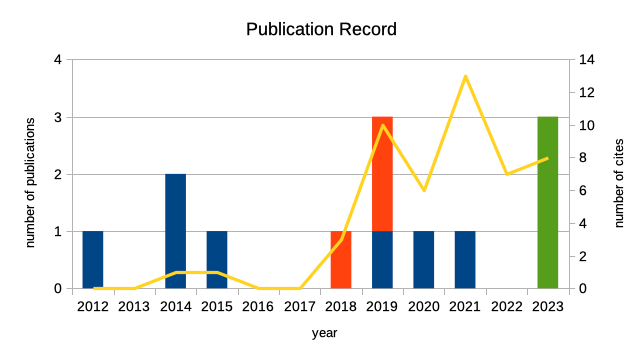
\includegraphics[width=9cm]{./images/publication-record.png}
\caption{{\color{RedOrange}$\lgblksquare \ $} journal articles; {\color{RoyalBlue}$\lgblksquare \ $} conference article; {\color{LimeGreen} $\lgblksquare \ $} journal article in preparation; {\color{Goldenrod}$\lgblksquare \ $} citations.} \label{fig:publication-record}
\end{figure}

\begin{figure}[h]
\centering
\captionsetup{justification=centering}
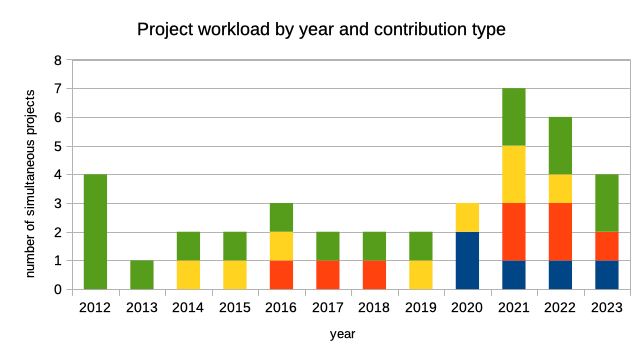
\includegraphics[width=9cm]{./images/project-record.png}
\caption{Project contribution type:{ {\color{RoyalBlue}$\lgblksquare \ $} Principal Investigator and 
project development; \color{RedOrange}$\lgblksquare \ $} Proposal writing and development; {\color{Goldenrod}$\lgblksquare \ $} Full development; {\color{LimeGreen} $\lgblksquare \ $}: Partial development.} \label{fig:project-record}
\end{figure}

\subsection{Research Awards}
\begin{itemize}
\item {\bf 2022:} 2022 HPC Innovation Excellence Award from Hyperion Research. Total awarded amount: 1.000,0€ \hyperlink{hyperion-award.1}{(see ref. letter)} 
\end{itemize}

\newpage
\section{Academic, Research, and Professional Record Description}

I started my professional career in 2001 while studying for a Master's in Industrial Engineering (thermal and mechanical majors) at the Technical University of Catalonia (UPC), which I finished in 2003 \hyperlink{carrera-EI.1}{(see document)}. Since then, I have developed my career in a wide variety of environments, which allowed me to acquire an uncommonly broad vision of scientific and technological development in the Fluid Mechanics, Thermal, and Mechanical fields, from a fundamental research perspective to the practical industrial application. Specifically, I worked in large and medium-sized industrial private companies (NISSAN Motor Company and Carandini), in a technological spin-off company (TermoFluids), in university research centers (UPC, Massachusetts Institute of Technology), and in a leading public research center (Barcelona Supercomputing Center). Below, a more detailed overview of my academic and professional evolution is given:

In 2001 I started teaching in a university preparatory academy (Acadèmica Blancafort) during the final years of my Master's degree, teaching Mathematics, Physics, Technology, Mechanics, and Electrotechnology.
Later, in 2005, I started working in the private industrial sector as an R\&D engineer at the NISSAN Motor Company in the Engine Installation Department \hyperlink{nissan.1}{(see ref. letter)}. In this position, I got my first contact with numerical simulation of thermal and mechanical industrial problems. This was one of my responsibilities, among many others, that gave me a deep understanding of the whole development pipeline of a thermal-engine-based vehicle, from the first design and prototyping stage to the start of production. 
Then, in 2008, I moved to C\&G Carandini to further expand my knowledge of numerical simulation with other modeling tools and technical challenges \hyperlink{carandini.1}{(see ref. letter)}. In total, I gathered more than five years of experience in the private industrial sector, in which I widely used numerical simulation tools, becoming aware of their potential in technological development. 

To gain more insight into the numerical simulation fundamentals, in 2010, I studied for a Master's in computational methods applied to thermal and fluid mechanics problems at the UPC \hyperlink{master-E.1}{(see document)}. This experience allowed me to join Termofluids (end of 2011), a company focused on multiphysics simulation software \hyperlink{termofluids.1}{(see ref. letter)}. The company was a spin-off of the UPC's Heat and Mass Transfer Technological Center (CTTC).
My role in the company was a combination of Industrial Ph.D. student on physical and computational models for fluid dynamic problems, software developer of the parallel C++-based in-house code, and project developer. In my position as a researcher, I started a new  research line from scratch on wall modeling for Large Eddy Simulation (WMLES) to allow high-Reynolds aerodynamic simulations of industrial-relevant applications.  I also carried out the full development of a clean-sky European project related to turbomachinery for aeronautical applications, among other projects \hyperlink{projectes-tf.1}{(see ref. letter)}. 

 In 2017 I moved to the CTTC at UPC to focus exclusively on research aspects and finish my Ph.D. This is reflected in my CV since most of my journal publications were published in this more academic-oriented period (see Fig. \ref{fig:publication-record}).  \hyperlink{projectes-cttc.1}{(see ref. letter)}
In parallel, to foster my research career and gain international experience, in 2017, I completed a four-month doctoral stay at the Aerospace Computational Design Laboratory (ACDL) at Massachusetts Institute of Technology with Prof. Jaume Peraire \hyperlink{mit.1}{(see ref. letter)}. At the same time, I also established a collaboration with Prof. Volkov, a visitor from Worcester Univ., from which a work was published. Moreover, I also participated in several lectures on Helicopters and Wind Energy subjects to teach fundamental aerodynamics and the use of the airfoil simulation code xfoil. 

In July 2019, I obtained my Ph.D. in Computational Science applied to Fluid Dynamics within the Thermal Engineering Doctorate Program \hyperlink{doctorat.1}{(see document)}. My Thesis was titled «Efficient Wall Modeling for LES of General Non-Equilibrium Wall-Bounded Flows.» An international committee awarded the Thesis the maximum qualification of Excellent cum laude and International Mention.

In Nov. 2019, I joined the Large-Scale CFD (LSCFD) group at the Barcelona Supercomputing Center as a postdoctoral researcher. \href{https://www.bsc.es/discover-bsc/organisation/research-departments/large-scale-computational-fluid-dynamics}{(LSCFD website)}. 
My initial responsibility at the LSCFD was to open a new research line in flow and pollutant transport phenomena prediction in urban environments from scratch. I initially applied WMLES strategies to model urban flow and pollutant dispersion. Nevertheless, the explosion of Artificial Intelligence and its application to solve fluid dynamic problems deeply aroused my curiosity. For this reason, in October 2020, I enrolled a postgraduate program in Deep Learning at the UPC to learn the fundamentals of the most advanced techniques in the area \hyperlink{postgrau-DL.1}{(see document)}. Since then, I reoriented my research focus to applying those techniques to different fluid dynamics challenges allowing me to acquire a horizontal role within the LSCFD group by promoting the use of AI-based methods in all the group research lines. 
As a member of the LSCFD group, I devoted a significant part of my efforts to securing both financial and computing resources to develop the research lines in which I worked (see Figure \ref{fig:project-record}). In that sense, I wrote 6 competitive project proposals for public funding, from which 3 have succeeded, and one is still resolution-pending. The total funding provided by the projects amounts to around 1.1 million €, from which approximately 400 k€ for the BSC \hyperlink{projectes-bsc.1}{(see ref. letter)}. Moreover, I also wrote as a Principal Investigator 7 computing allocation project proposals, 5 of them successful, totaling an amount of more than 11 million CPU-h in computational resources, ensuring the project completion from a financial and computational resource point of view \hyperlink{projectes-res.1}{(see ref. letter)}. Moreover, I have also coordinated a team of two people, a Research Engineer and a Ph.D. student who participated in the project development. 

My current research lines have been or are being developed in the framework of European and National competitive projects \hyperlink{projectes-bsc.1}{(see ref. letter and} \href{https://futur.upc.edu/JoanCalafellSandiumenge/as/cGFydGljaXBhY2lvUHJvamVjdGVSRElDb21wZXRpdGl1}{ Futur UPC)}, which revolve around the use of advanced AI techniques to tackle fluid mechanic and passive-scalar transport challenges from a fundamental and applied point of view. One of the projects has been an innovation success and was awarded the 2022 HPC Innovation Excellence Award from Hyperion Research \hyperlink{hyperion-award.1}{(see ref. letter 1)} \hyperlink{carta-bettair.1}{(see ref. letter 2)}. The scientific results of this project are being gathered in two articles. However, due to legal restrictions imposed by the industrial partner, the results cannot be published until one year after the project end (Sept. 2023). I am also participating in the NextSim project intended to develop the next generation of aerodynamic simulation code for Airbus together with Onera, Cerfacs, DLR, and UPM. 

In September 2022, I started as an assistant professor (Professor Associat) at UPC. Specifically, I have been teaching Thermal Machines theory (Màquines Tèrmiques, 240EI021, 4.5 ECTS), a core subject of the Master in Industrial Engineering (MUEI) at the "Escola Tècnica Superior d'Enginyeria Industrial de Barcelona" (ETSEIB) in the fall and spring terms of the 2022-2023 academic period. This subject requires a deep understanding and application of several major fundamental disciplines, namely, Fluid Mechanics, Heat Transfer, Thermodynamics, and Mechanics. On the other hand, I also participated in the creation of new laboratory sessions.
I really enjoyed teaching the subject, and I made a great effort to explain the subject contents as clearly as possible. This effort is reflected in the student satisfaction survey, where I obtained a 4.88 and a 4.75 score out of 5 on the two survey questions, respectively \hyperlink{enquestes.1}{(see ref. letter)}. 
Later in February 2023, I also started to teach Heat Transfer theory and numerical lab sessions (Termotècnia, 240171, 6 ECTS), a core subject of the Industrial Engineering Degree (GETI) at ETSEIB. The student satisfaction survey for this period is not available yet. 

As part of my teaching activity, since 2019, I have been advising the Ph.D. student Sarath Radhakrishnan \hyperlink{tesis.1}{(see ref. letter)} in his research. His work is related to machine learning-based wall models for Large Eddy Simulations. An article containing the research findings is being written and will be submitted to a Q1 journal in the coming months.  On the other hand, I have also supervised two final degree theses. The first was titled "Discovering new scaling laws in turbulent boundary layers via Multi-Expression Programming." My second co-directed work is titled "Autoencoders for fluid flow data compression", and it is still ongoing. Finally, I have also been a member of two Ph.D. thesis research plan committees \hyperlink{tribunals.1}{(see ref. letter)}.

In May 2023, I obtained the ANECA accreditation for an assistant professor ("Acreditación Ayudante Doctor"). Although it was a preferential merit for the present competitive recruitment process, I could not submit the accreditation documentation before the first call deadline since {\bf the ANECA resolution was released only three days after the submitting process expired} \hyperlink{acreditacio.1}{(see document)}.

As with collaborations, I still keep close ties and contacts with the places where I did my Ph.D., visits, and postdocs, as well as with the vast number of project partners I had during my research career. I am keeping these collaborations active for research and to be able to apply for competitive projects with them.  

\newpage
\section{Adequacy for the position}

My academic and professional record is very well suited for the positions opened in both research and lecturing. First, I have broad experience in computational and data-driven methods for fundamental and applied fluid mechanics, the two main areas specified for the position. My knowledge background is clearly Fluid Mechanics. In the academic aspect, I have several publications on computational aerodynamics (two in Q1 journals), and I will submit three publications on data-driven methods for fluid mechanic applications soon. During the iBAM and APPWIND projects, I was also involved in designing the experimental measurement campaigns to obtain validation data for the AI-based models, the third of the specified position topics. Moreover, I have one year of experience as a lecturer on the Thermal Engine and Heat Transfer core subjects. The Thermal Engine subject touches on many fundamental disciplines, primarily Thermodynamics, Fluid Mechanics, Heat Transfer, and Mechanics. I taught the theoretical part of the subjects, and I participated in designing laboratory sessions for the thermal Engine subject. On the other hand, I have ten years of experience in competitive project proposal writing and development related to computational and data-driven fluid mechanics (UCDLab,iBAM,APPWIND,MAESTRO,NextSim) and turbomachinery numerical simulation (EFFAN). 

It should be pointed out that:

\begin{itemize}
\item My academic and professional experience in a broad variety of environments, both academic and industrial, allows me to have an uncommonly global perspective of the technological development chain of applications involving Fluid Mechanics, Heat Transfer, and Thermodynamics. In recent years, I focused on solving fundamental and applied fluid mechanics, heat, and mass transfer problems through computational and AI-based methodologies, an exciting research field that deeply attracted me and on which I am willing to focus my research efforts in the near future. In that sense, I would be eager to integrate into a research group on these topics in order to create synergies and boost the group's scientific level and production. 

\item I have 3 journal publications in Q1 journals. However, I want to stress that I have prioritized targeting quality rather than quantity. Moreover, I also have seven conference articles and eleven oral presentations at international conferences. At present, I am writing three journal papers that gather the results of recently completed competitive projects. Two of them cannot be published until the end of the current year due to confidentiality restrictions. On the other hand, I have written three successful competitive funding projects by the BSC side, which amount to around 1.1 million € in competitive financing (400k€ for the BSC). Moreover, I have also written eight competitive computing allocation projects which provided 15 million CPU-h in computational resources, five of them as PI. In total, I participated in developing 21 competitive projects.

\item I have lecturing experience in the specific areas of the present position, Heat Transfer and Thermal Machines, which involves several fundamental disciplines such as Fluid Mechanics (convection) and Thermodynamics (Thermal Machine cycles). Moreover, the fundamental principles of steam and gas turbines could be easily adapted to hydraulic turbomachinery. On the other hand, I want to emphasize that I really like lecturing. Despite having a highly-demanding researcher position at BSC, I choose to continue lecturing as a part-time professor with a current teaching load of 6 hours per week.

\item I have always been curious to learn the most recent technological and methodological advances and stay updated. In that sense, my recent studies on advanced deep learning offered me the possibility of applying these techniques to all my research fields, making possible the development of new models and applications that were unfeasible so far, such as the fast flow and transport predictive tools. The range of applications of these methodologies is massive, and there is still a long way ahead in the opportunities that artificial intelligence can offer in Fluid Mechanics and its related areas. In that sense, the students should be given the opportunity to learn the fundamentals of these cutting-edge methodologies to later apply them to solve practical fluid mechanics-related problems, among others.      

\item I have the fundamental knowledge, technical skills, and management abilities required to successfully create and lead a research group and create an innovative teaching program to always provide students with the most advanced technological knowledge and methodological tools. My knowledge of computational fluid dynamics, heat and mass transfer numerical modeling, and thermodynamics is particularly well suited for the present position. This is also complemented by skills in HPC code implementation (C++, python, MPI, H5) for massive parallel solvers and data processing, HPC facilities use, and deep learning techniques for innovative modeling, among others. Finally, my skills in resource securing ensure the capability of achieving the proposed objectives from a financial and computational resources point of view.
\end{itemize}

\newpage
\section{Reference Letters and Supporting Documents}

\newpage
\thispagestyle{empty}
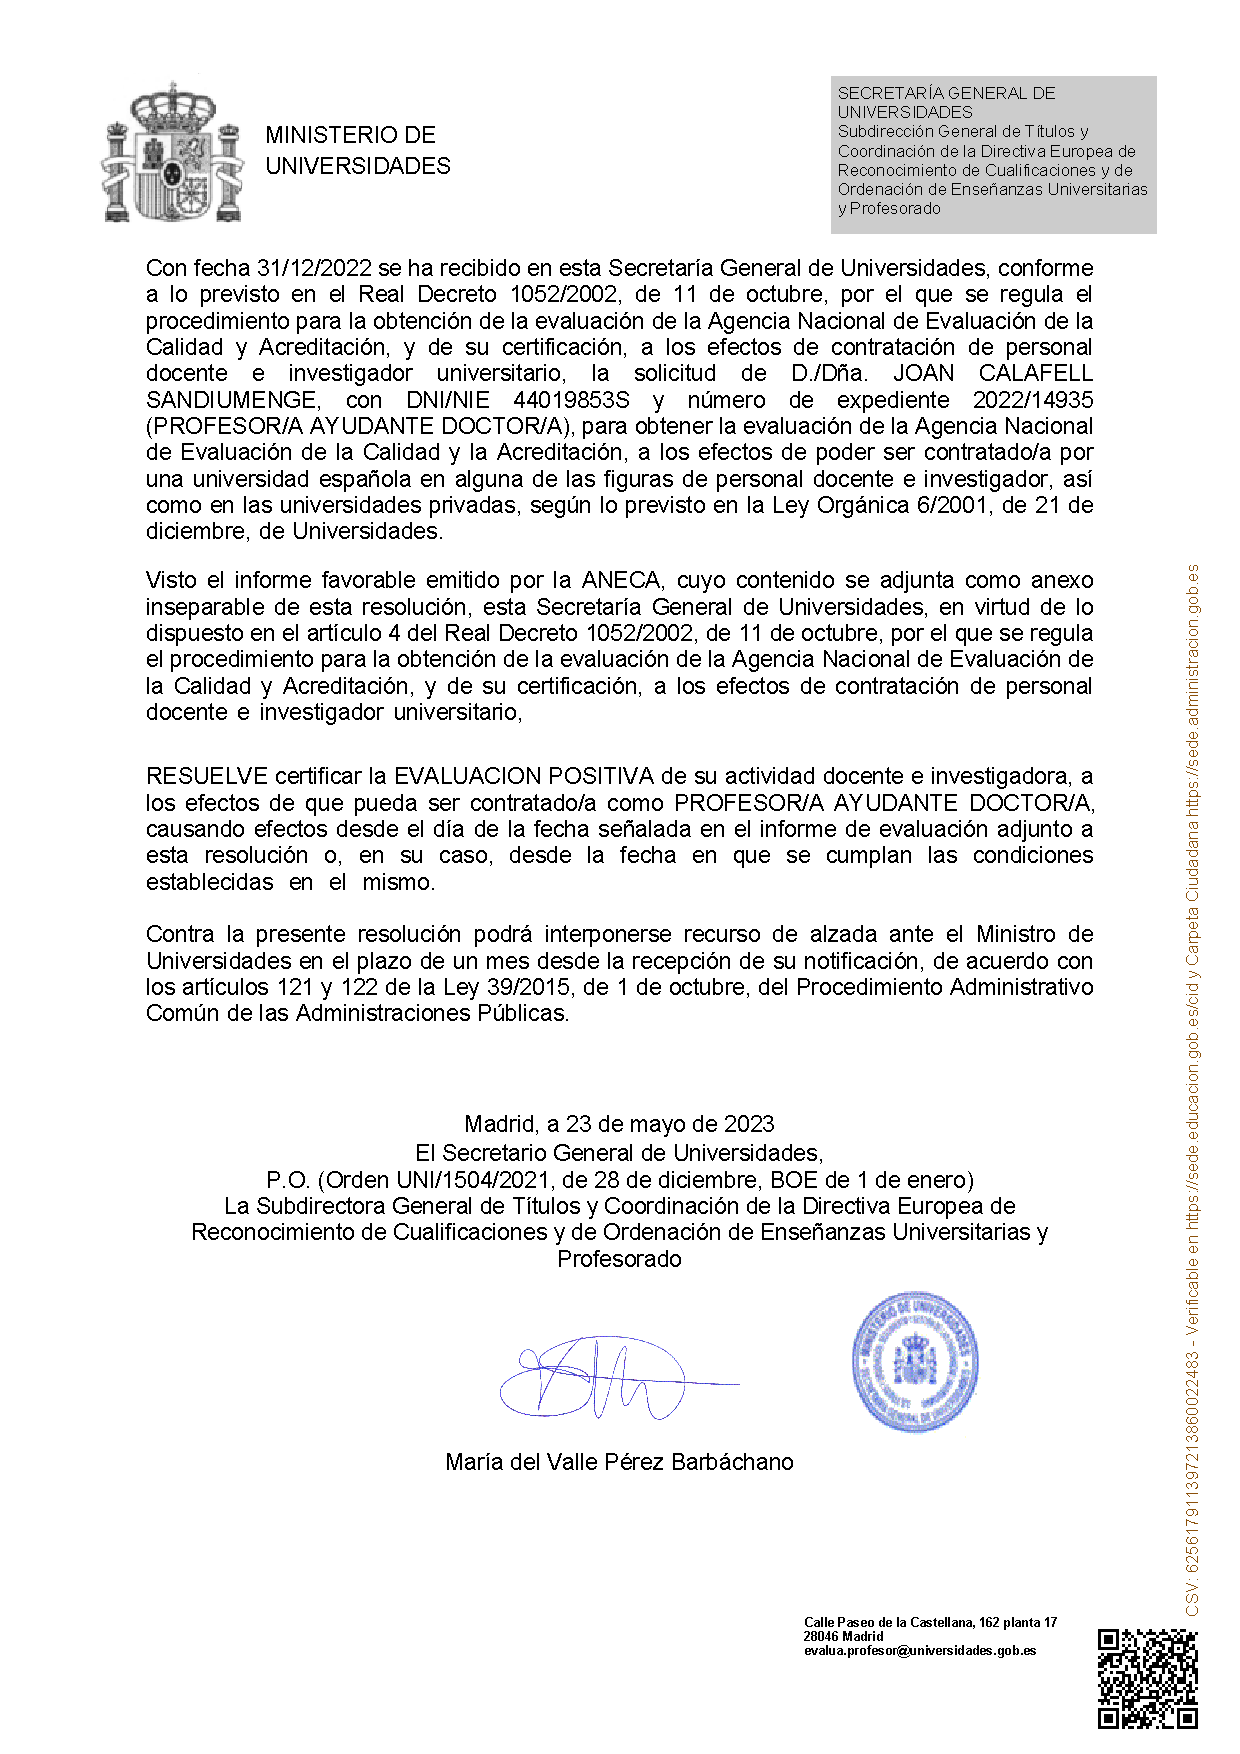
\includepdf[pages=-,link,linkname=acreditacio,pagecommand={\refstepcounter{includepdfpage}\label{testing.\theincludepdfpage}}]{./documents_justificacio/Calafell-Acreditacio-ANECA.pdf}
\thispagestyle{empty}
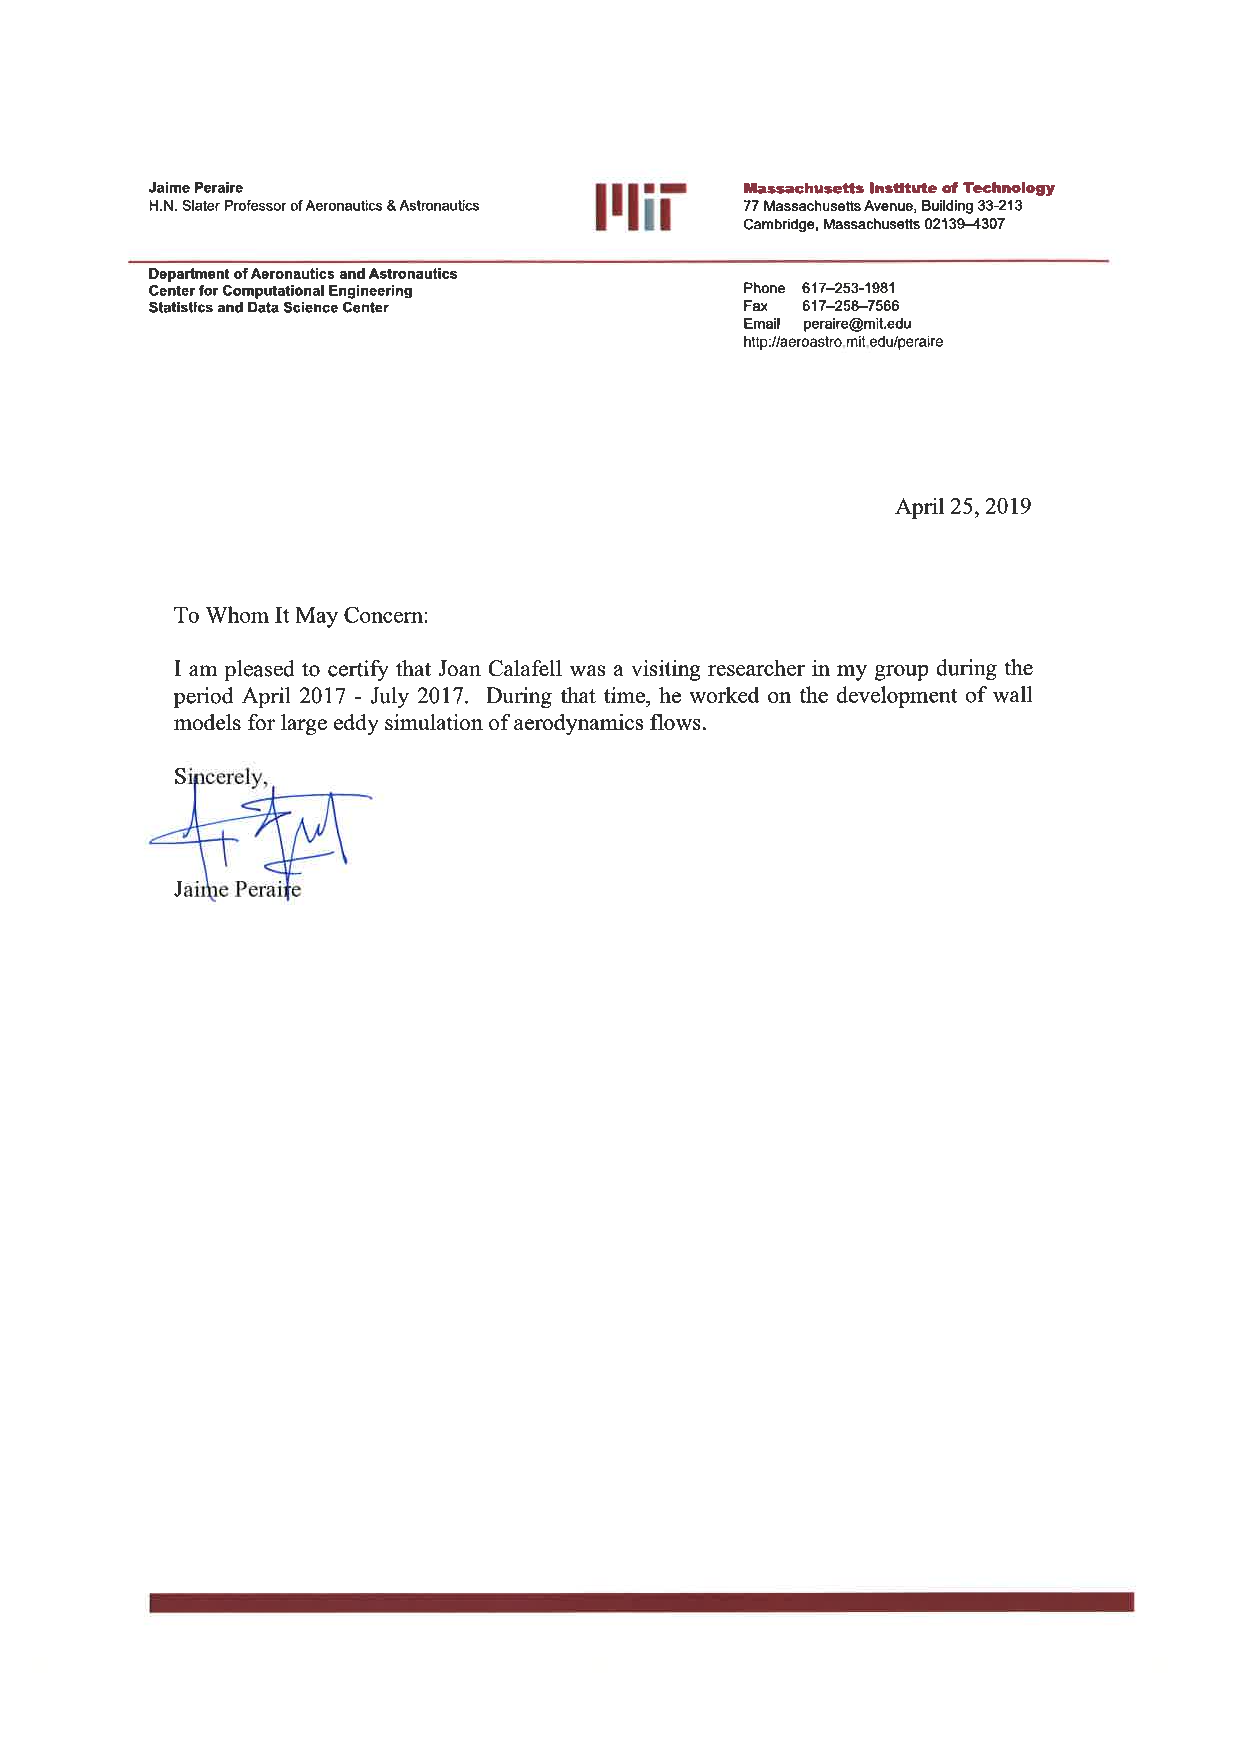
\includepdf[pages=-,link,linkname=mit,pagecommand={\refstepcounter{includepdfpage}\label{testing.\theincludepdfpage}}]{./documents_justificacio/Carta-Jaume-MIT.pdf}
\thispagestyle{empty}
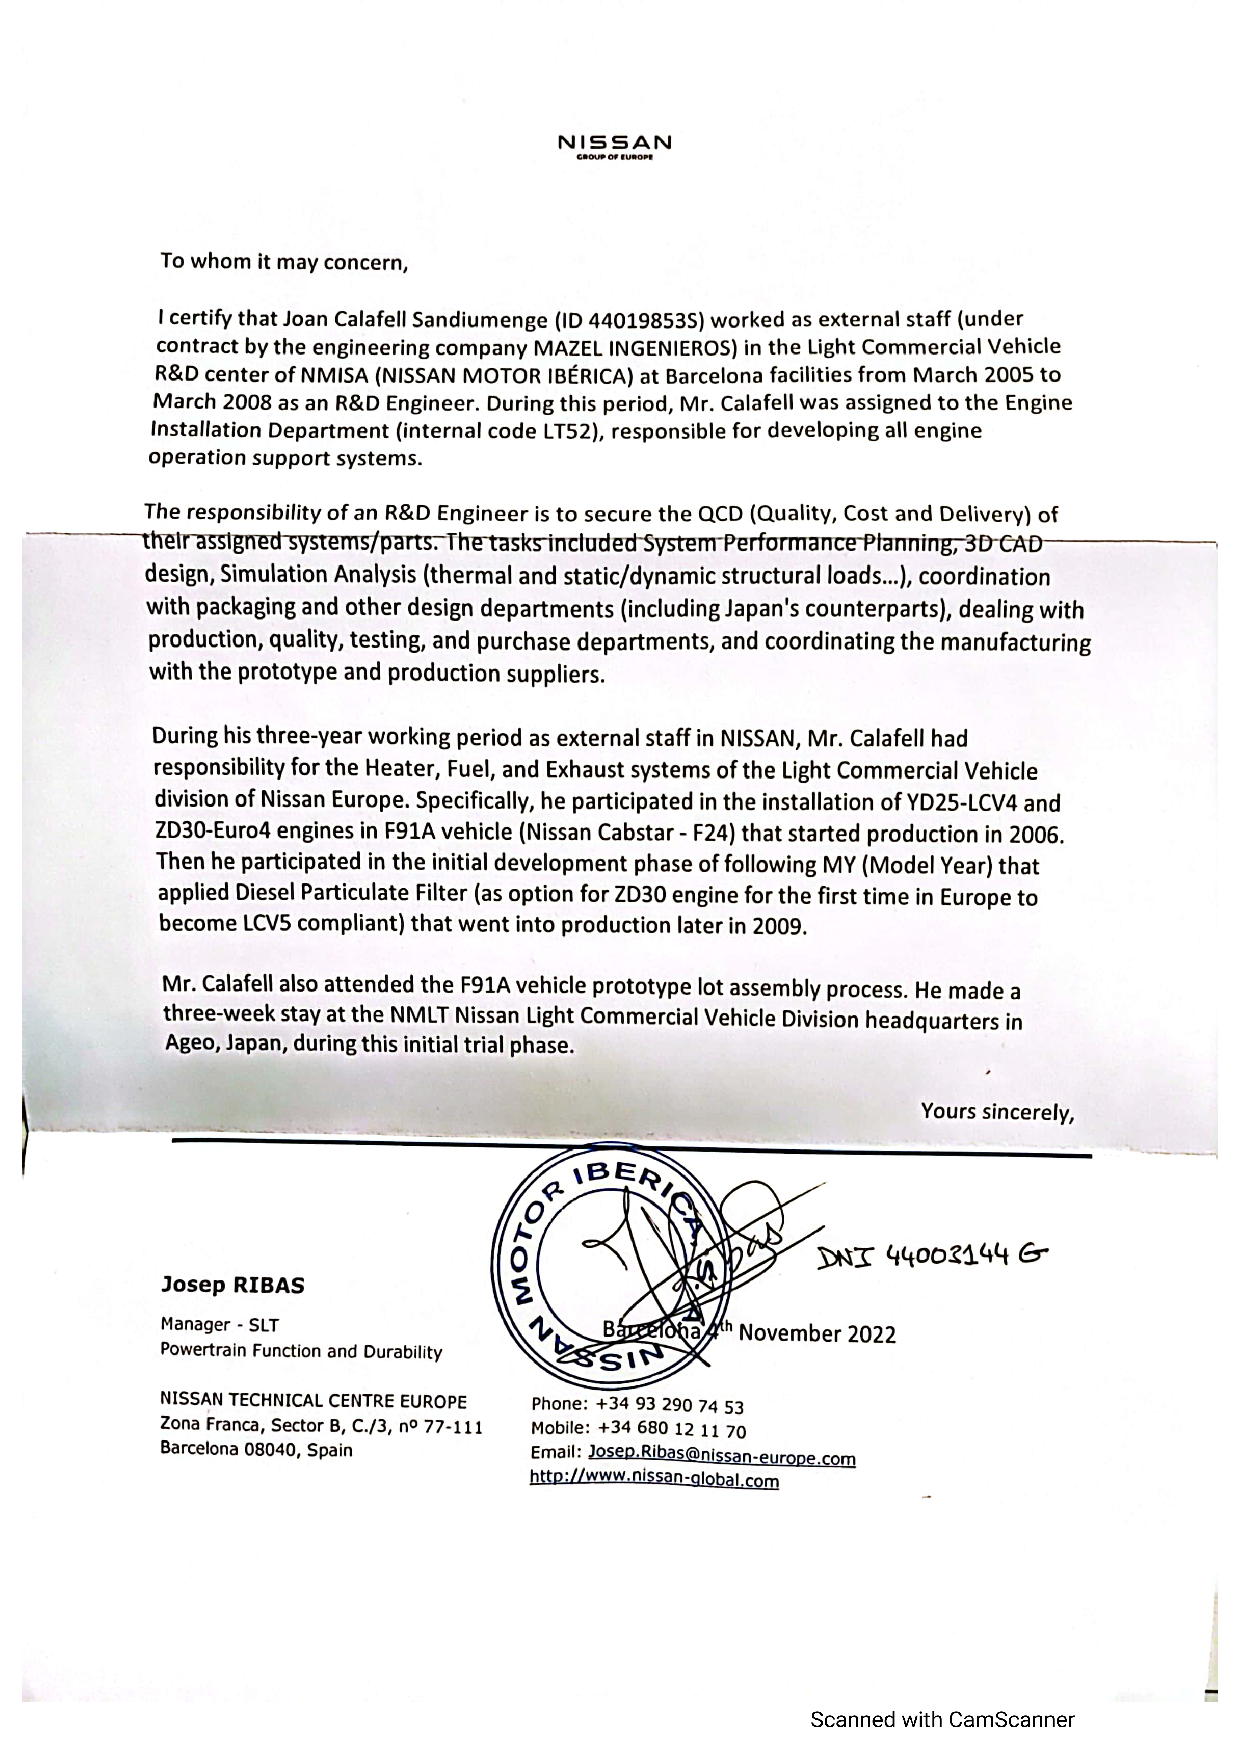
\includepdf[pages=-,link,linkname=nissan,pagecommand={\refstepcounter{includepdfpage}\label{testing.\theincludepdfpage}}]{./documents_justificacio/informe-NISSAN.pdf}
\thispagestyle{empty}
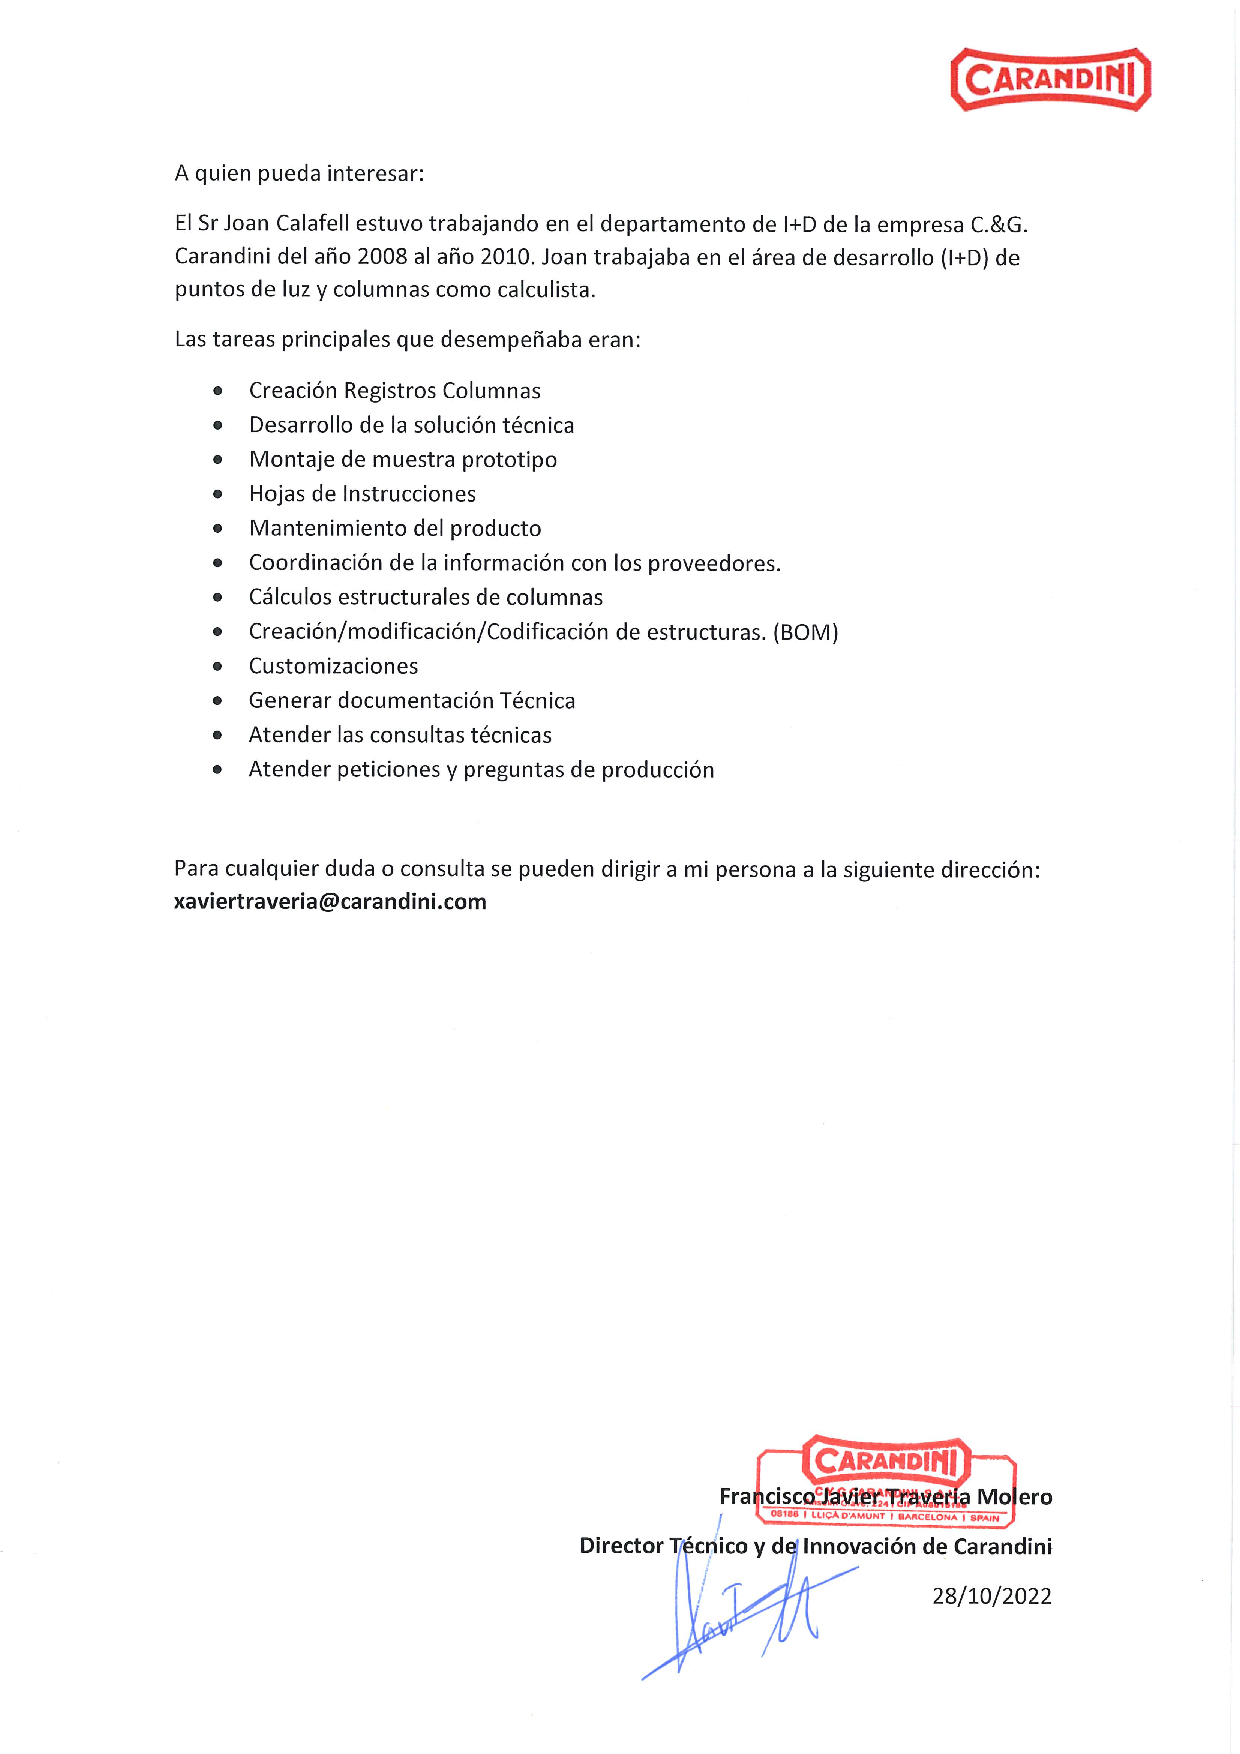
\includepdf[pages=-,link,linkname=carandini,pagecommand={\refstepcounter{includepdfpage}\label{testing.\theincludepdfpage}}]{./documents_justificacio/informe-CARANDINI.pdf}
\thispagestyle{empty}
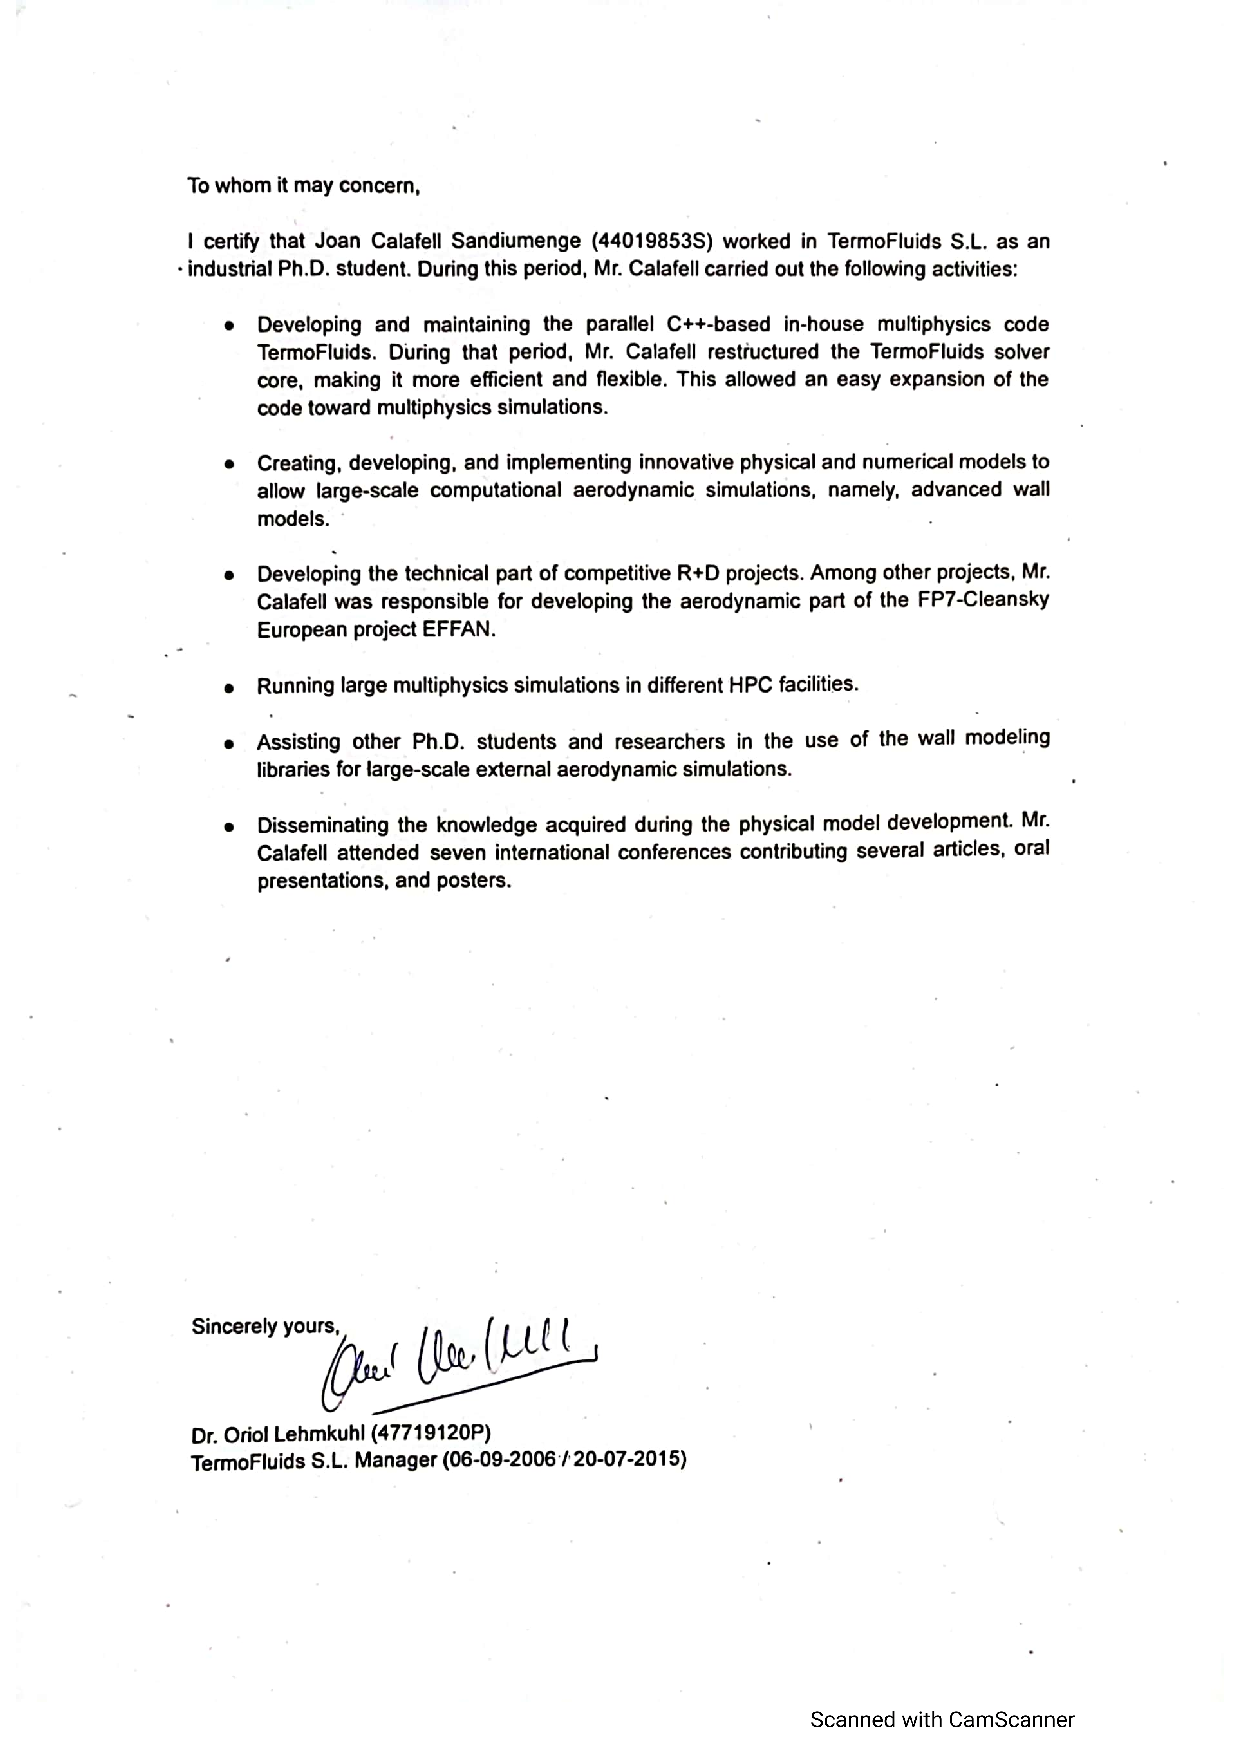
\includepdf[pages=-,link,linkname=termofluids,pagecommand={\refstepcounter{includepdfpage}\label{testing.\theincludepdfpage}}]{./documents_justificacio/informe-TermoFluids-noboe.pdf}
\thispagestyle{empty}
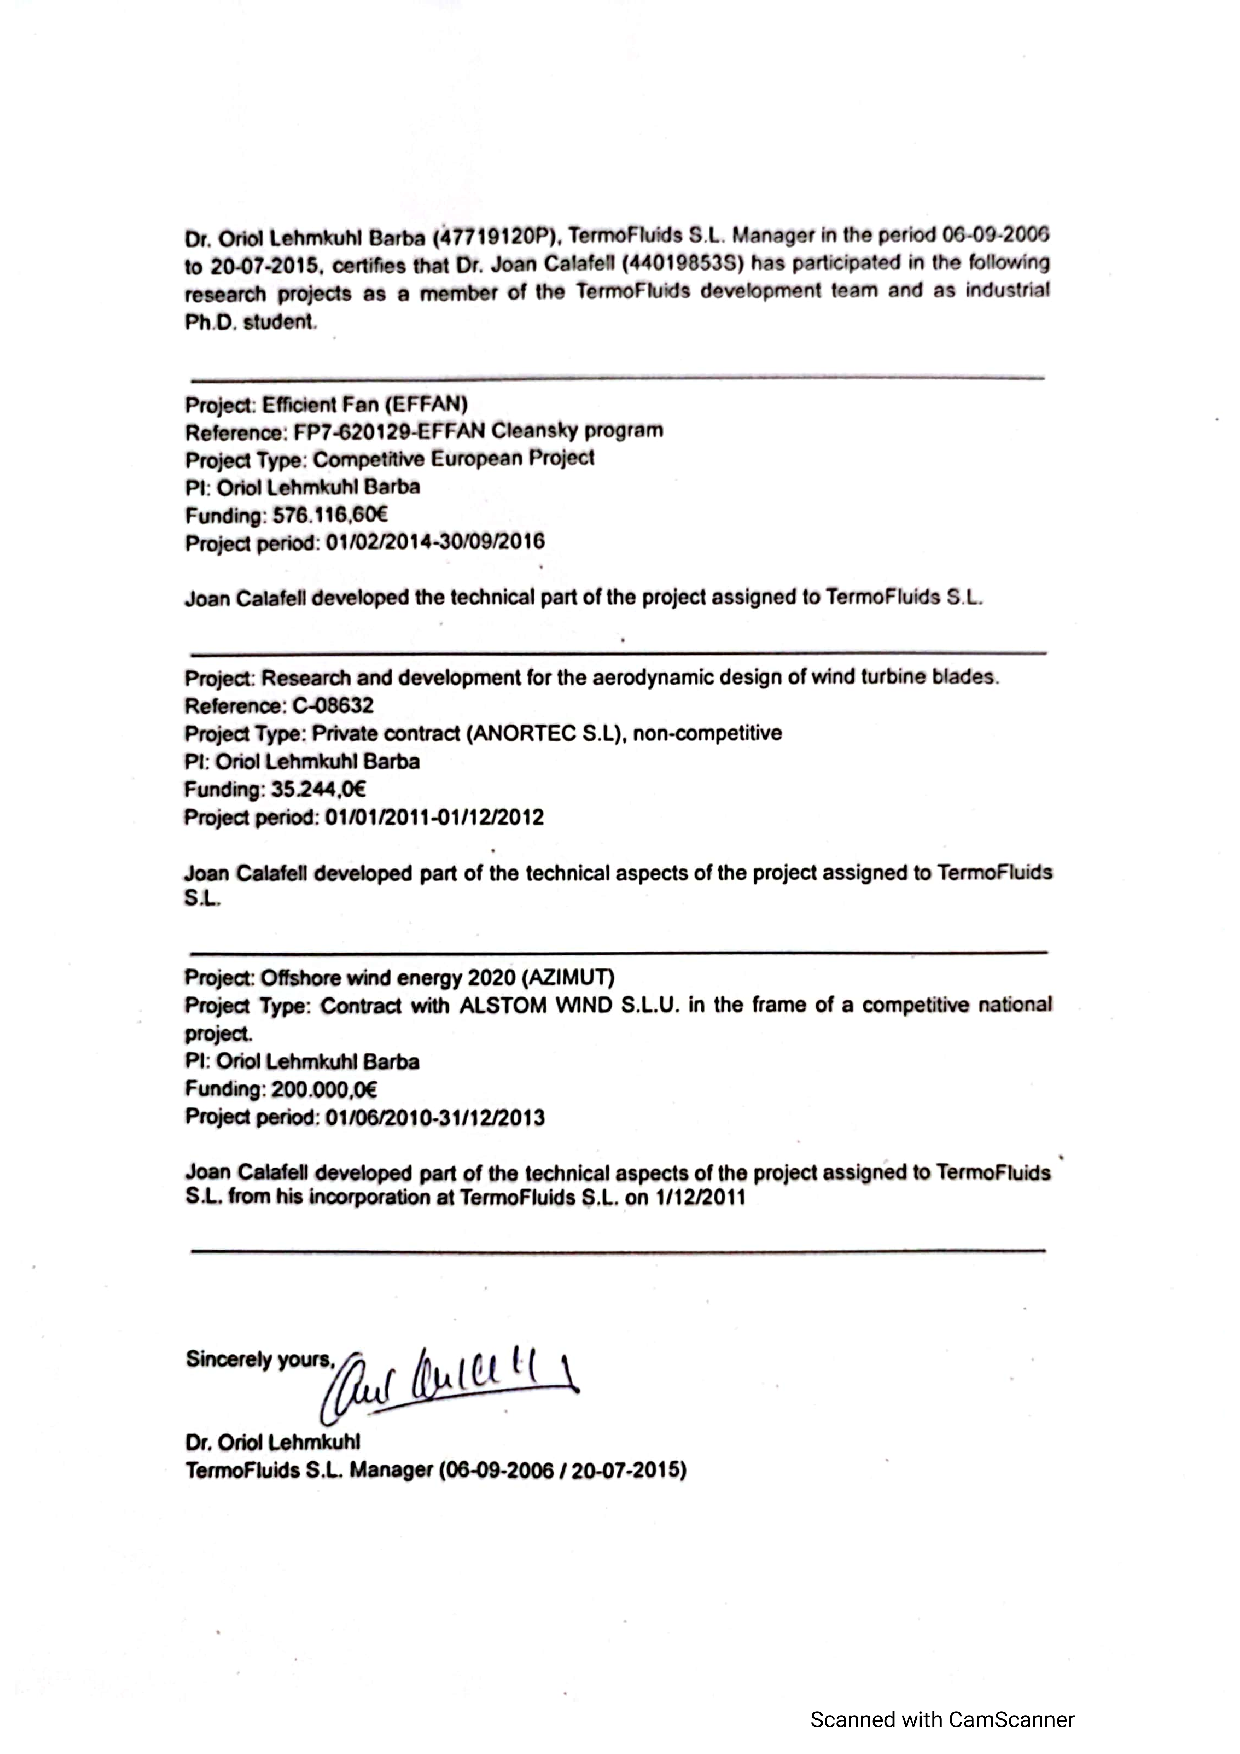
\includepdf[pages=-,link,linkname=projectes-tf,pagecommand={\refstepcounter{includepdfpage}\label{testing.\theincludepdfpage}}]{./documents_justificacio/Projectes-TermoFluids.pdf}
\thispagestyle{empty}
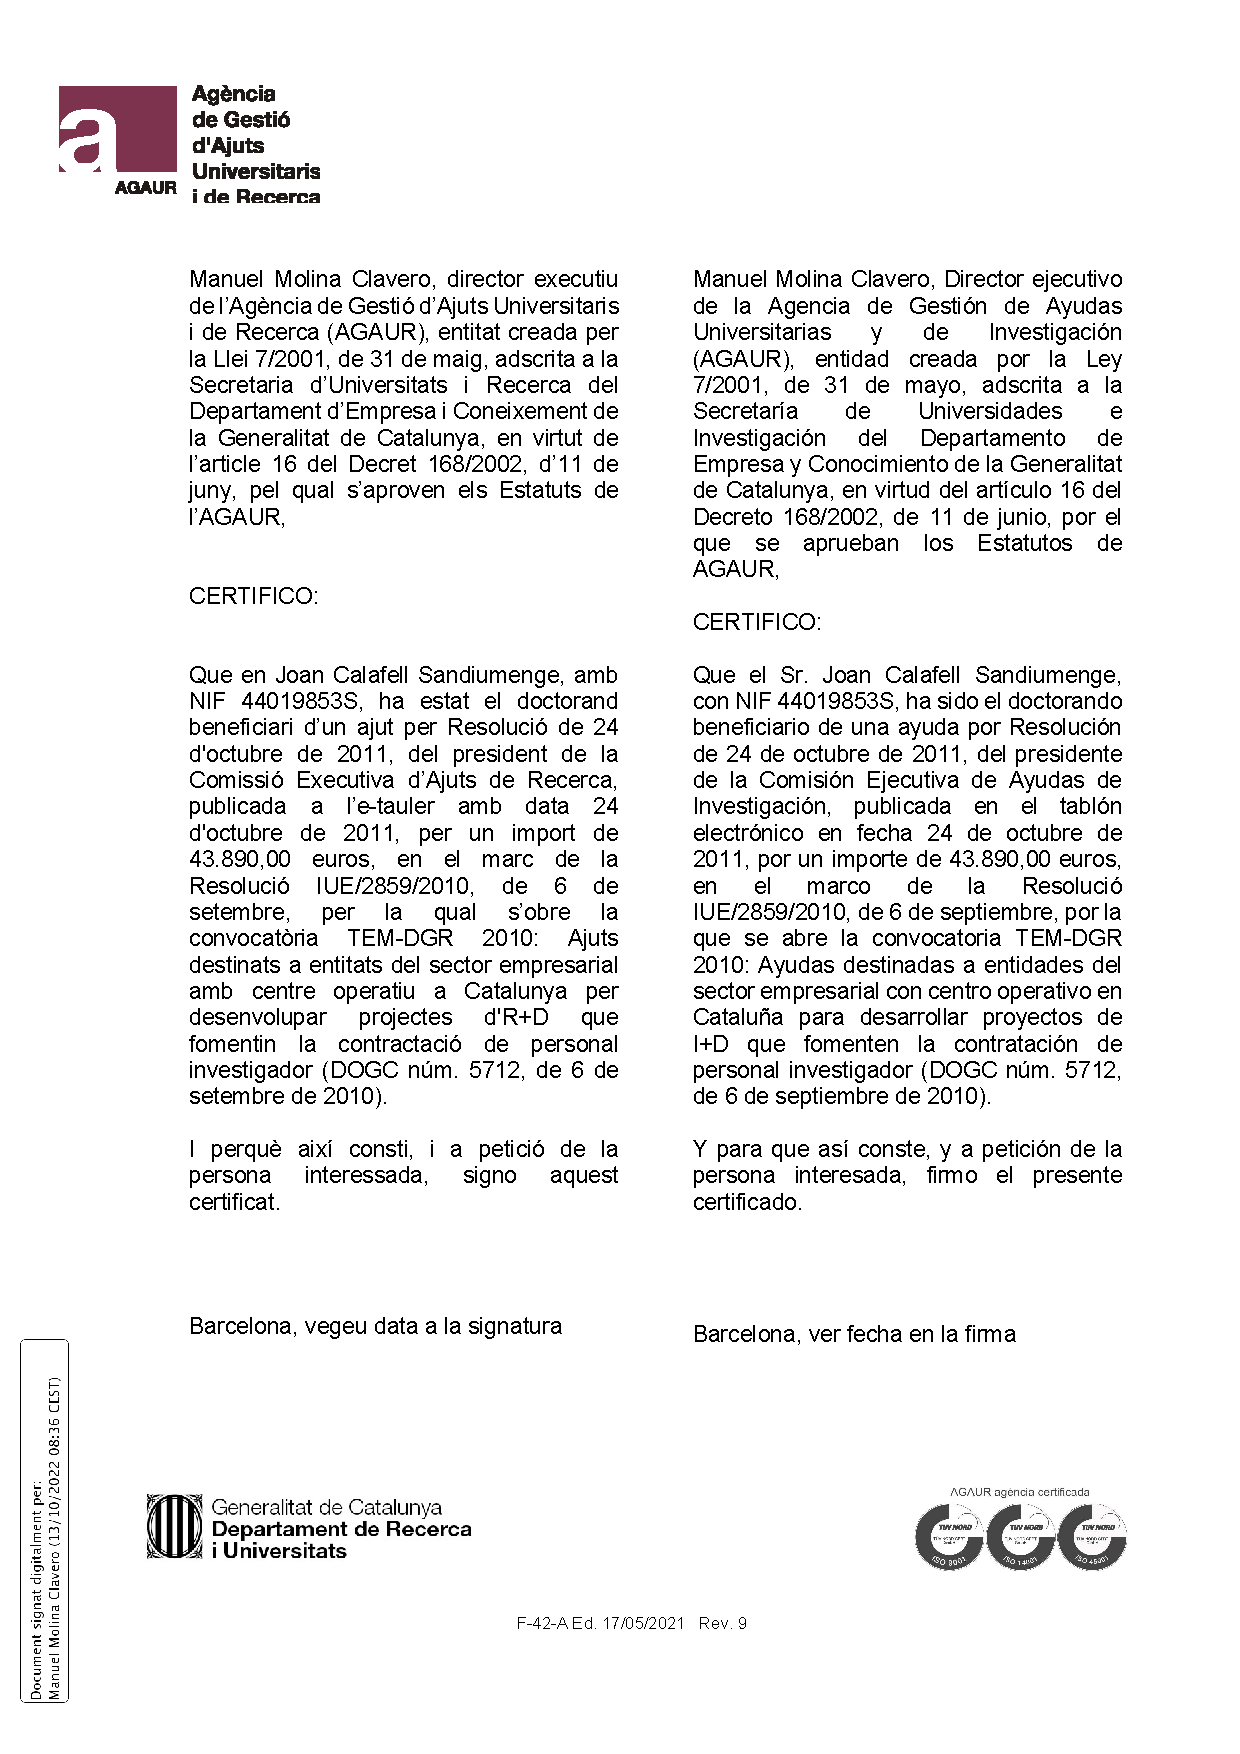
\includepdf[pages=-,link,linkname=agaur,pagecommand={\refstepcounter{includepdfpage}\label{testing.\theincludepdfpage}}]{./documents_justificacio/Calafell-agaur.pdf}
\thispagestyle{empty}
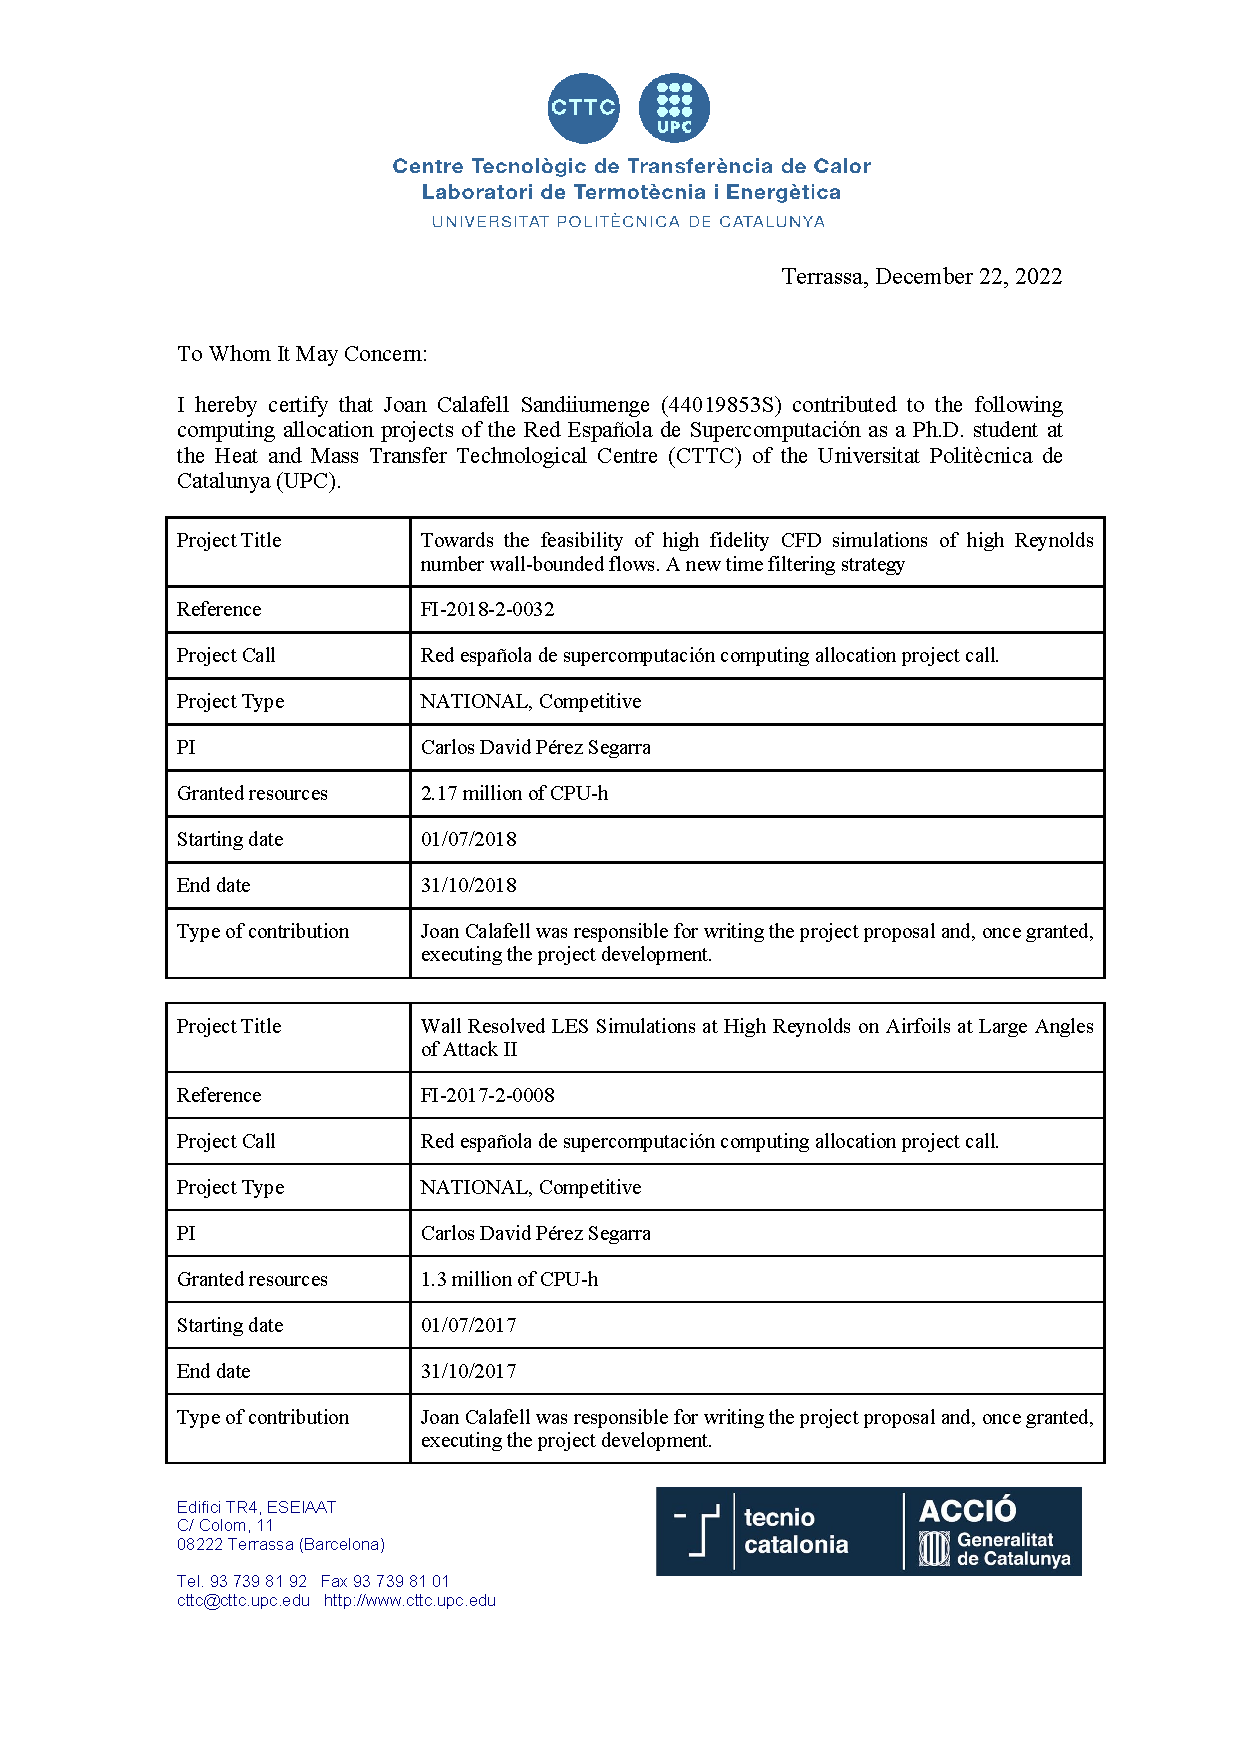
\includepdf[pages=-,link,linkname=projectes-cttc,pagecommand={\refstepcounter{includepdfpage}\label{testing.\theincludepdfpage}}]{./documents_justificacio/Projectes-CTTC.pdf}
\thispagestyle{empty}
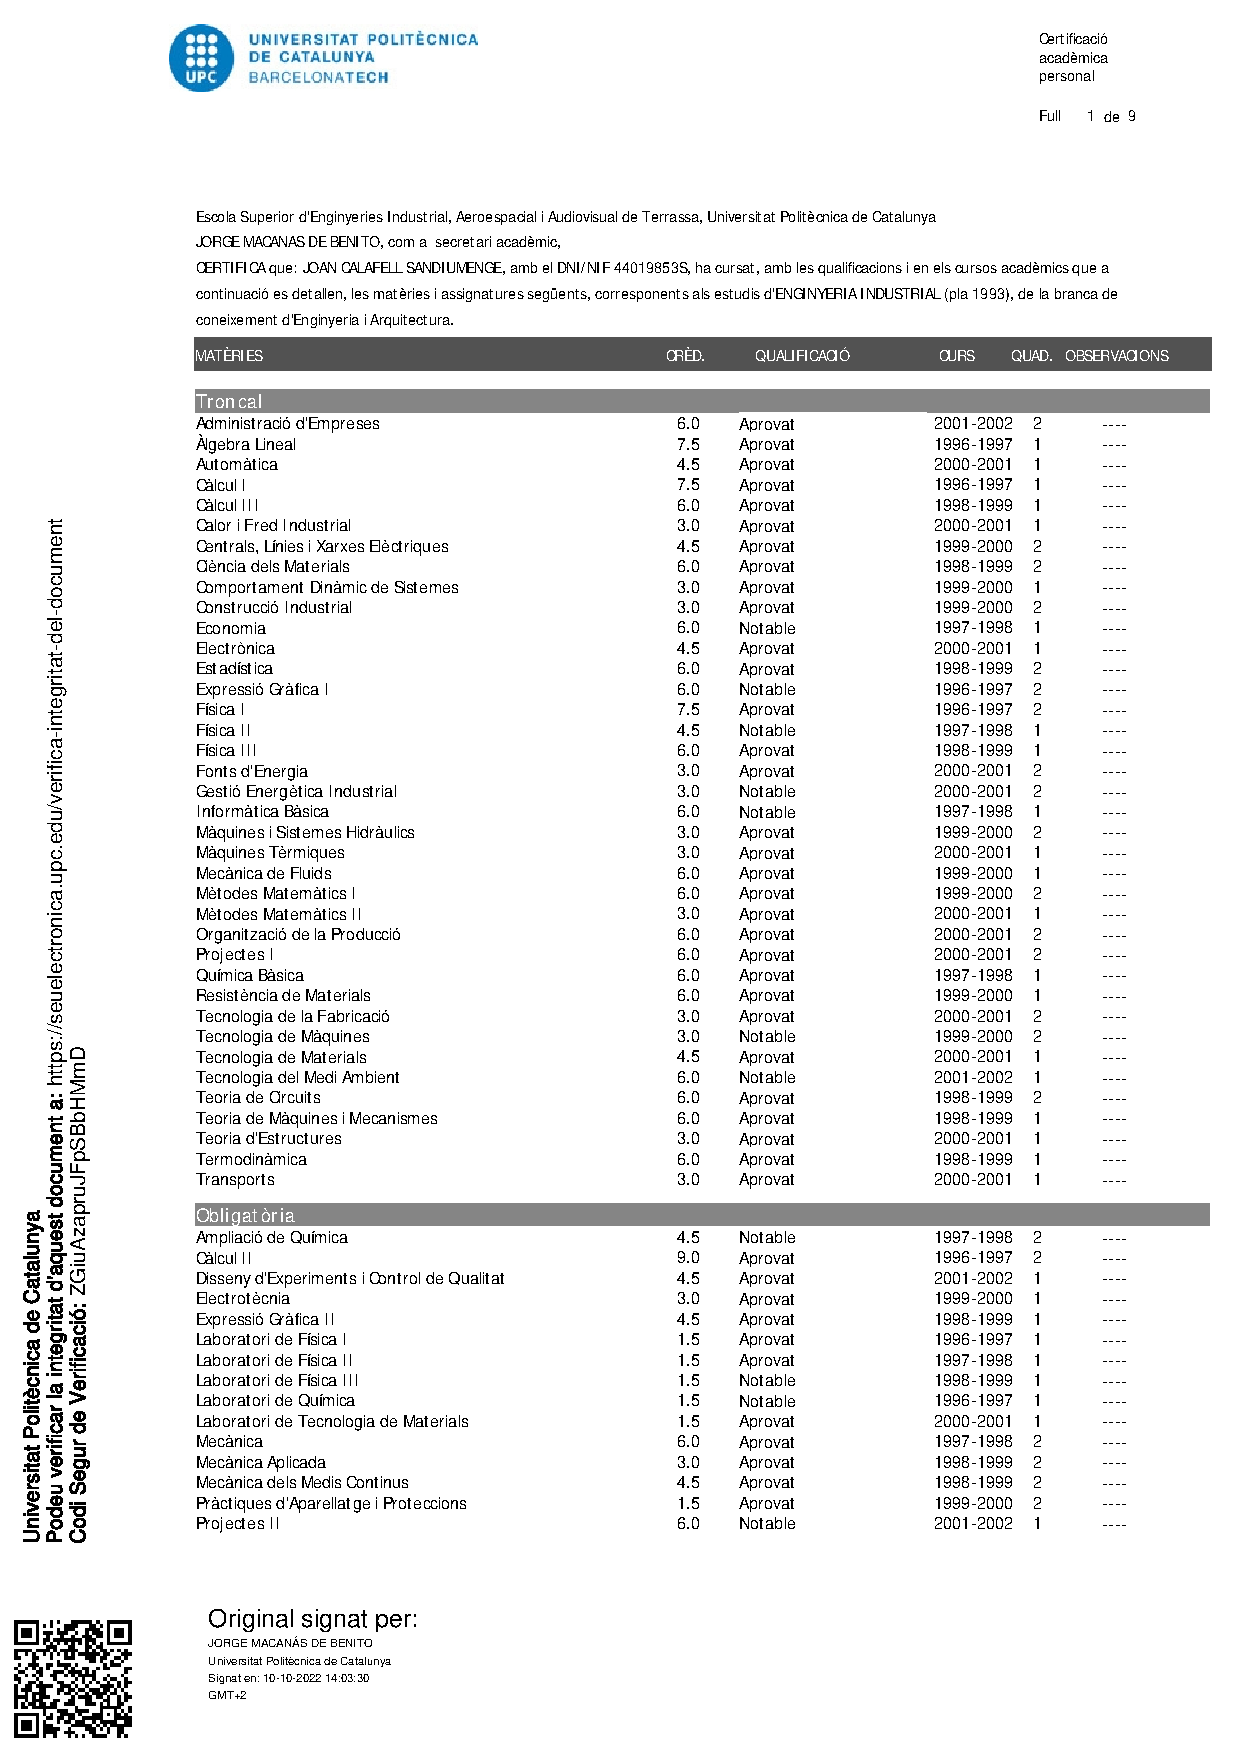
\includepdf[pages=-,link,linkname=carrera-EI,pagecommand={\refstepcounter{includepdfpage}\label{testing.\theincludepdfpage}}]{./documents_justificacio/Calafell-Certificat-Industrials.pdf}
\thispagestyle{empty}
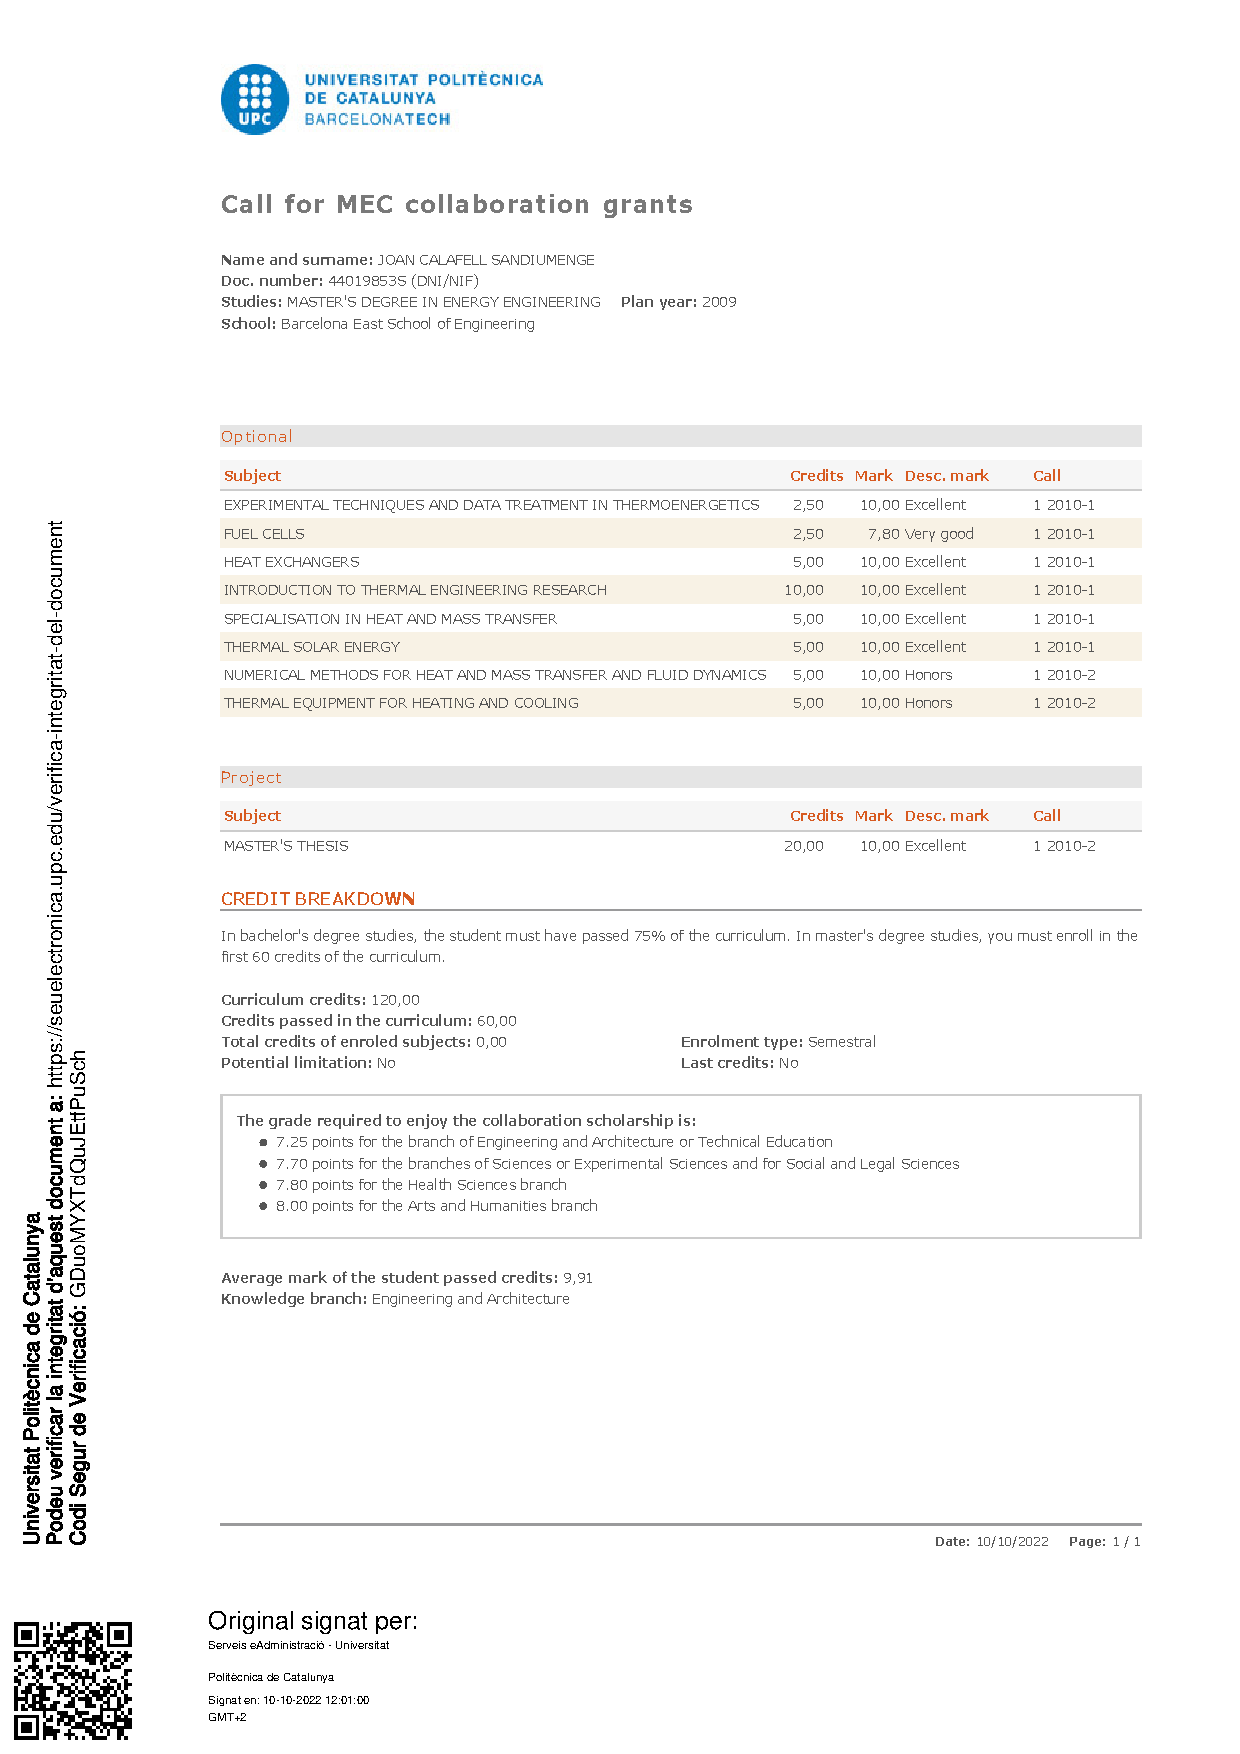
\includepdf[pages=-,link,linkname=master-E,pagecommand={\refstepcounter{includepdfpage}\label{testing.\theincludepdfpage}}]{./documents_justificacio/Master-Energia-Expedient.pdf}
\thispagestyle{empty}
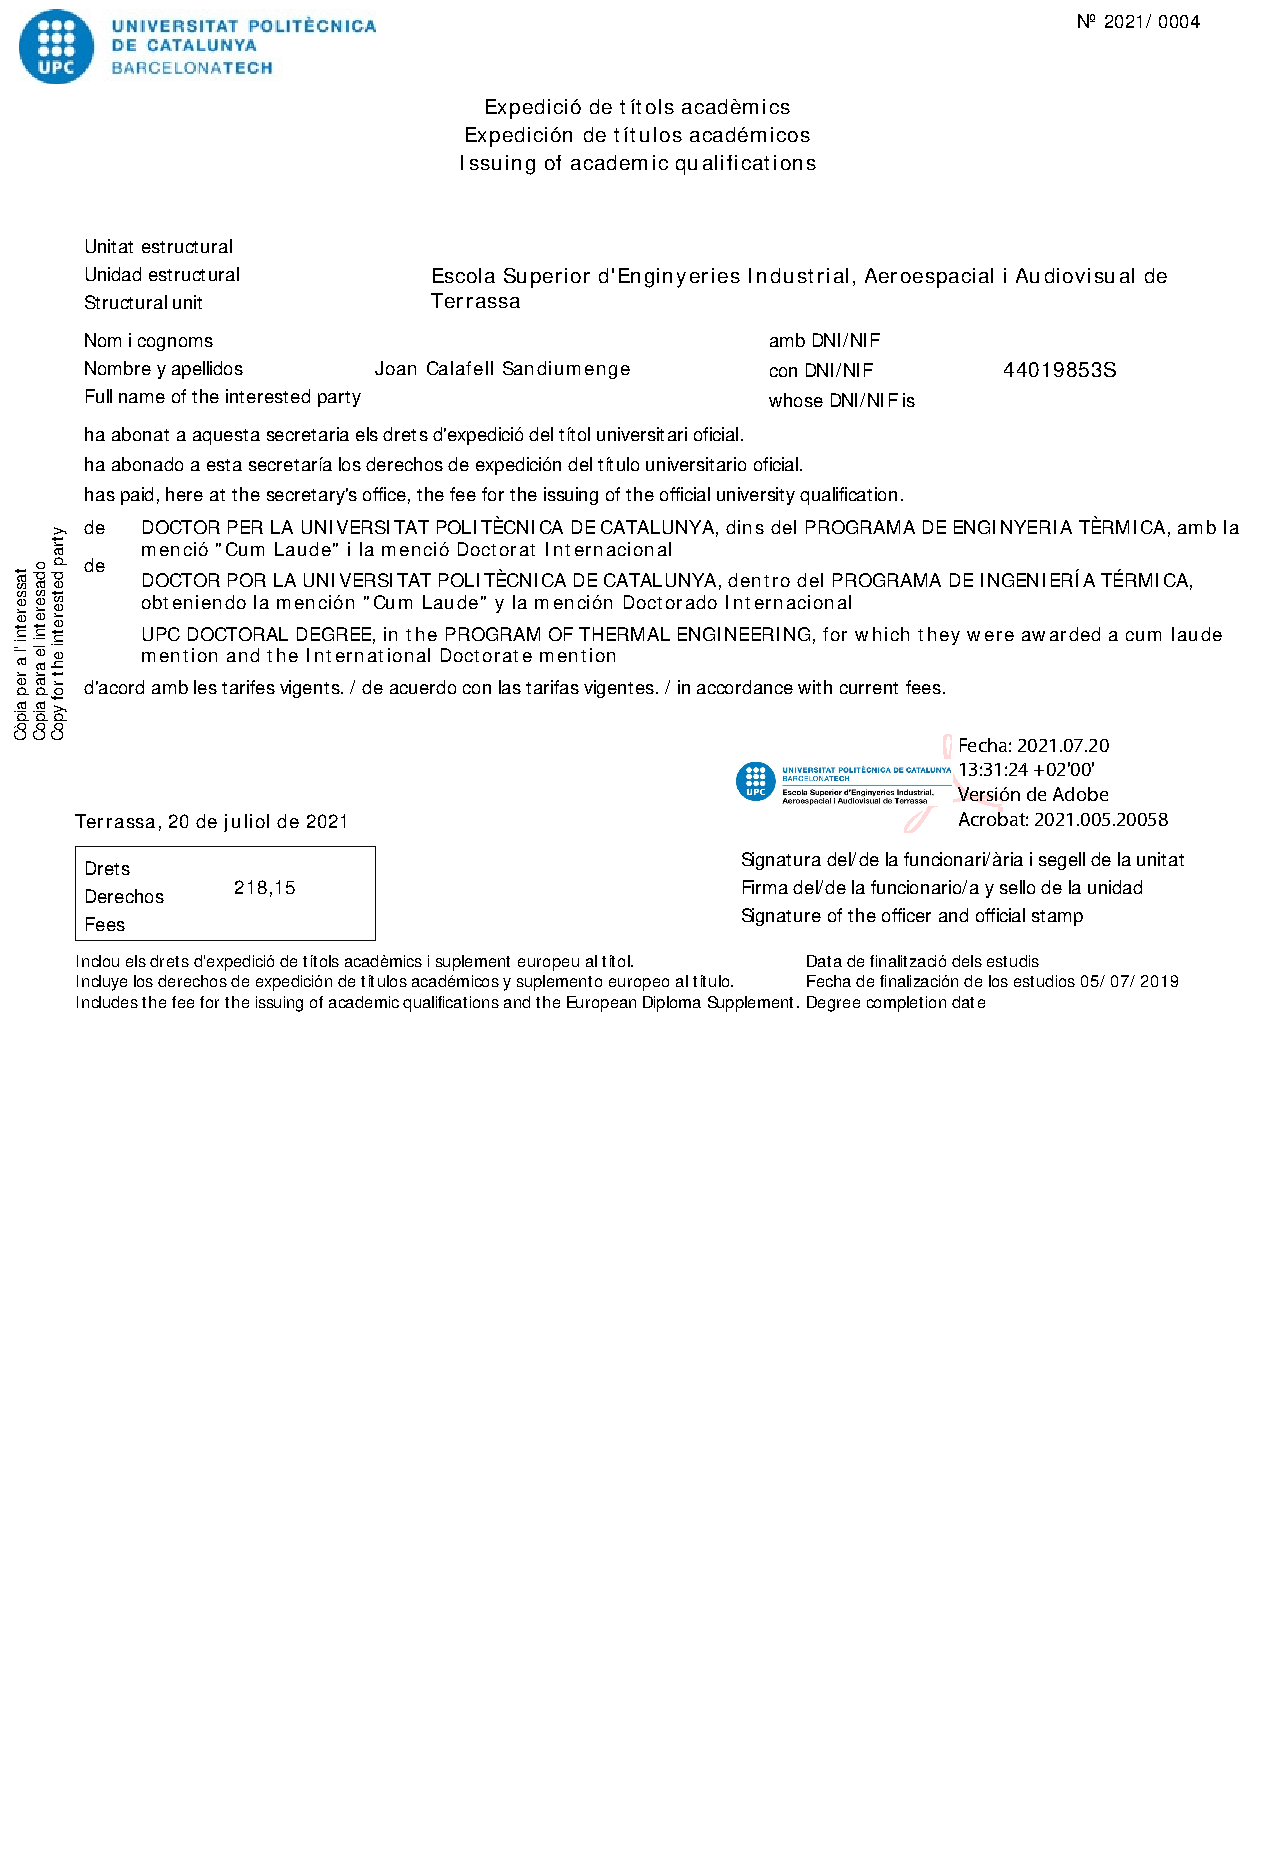
\includepdf[pages=-,link,linkname=doctorat,pagecommand={\refstepcounter{includepdfpage}\label{testing.\theincludepdfpage}}]{./documents_justificacio/2019-Titol-Doctor.pdf}
\thispagestyle{empty}
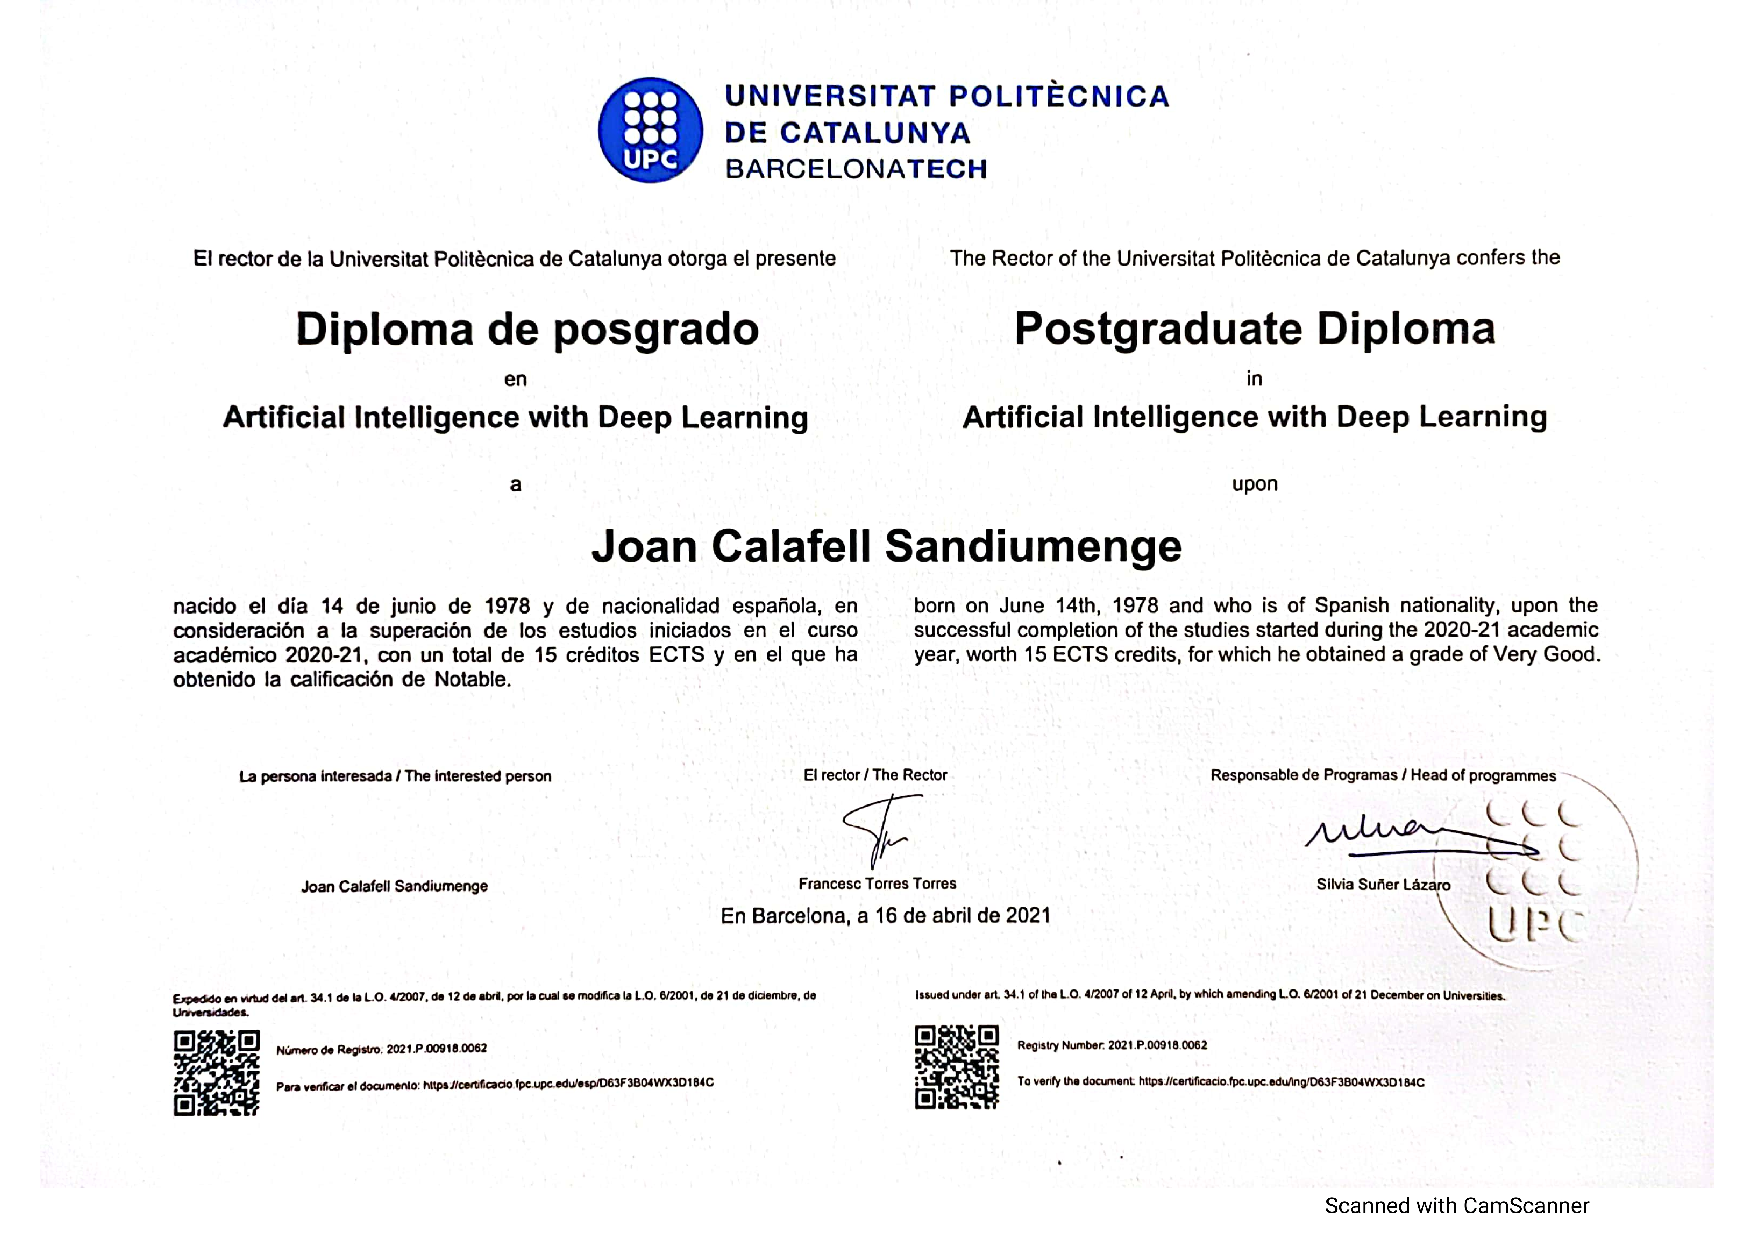
\includepdf[pages=-,link,linkname=postgrau-DL,pagecommand={\refstepcounter{includepdfpage}\label{testing.\theincludepdfpage}}]{./documents_justificacio/Postgrau-DL.pdf}
\thispagestyle{empty}
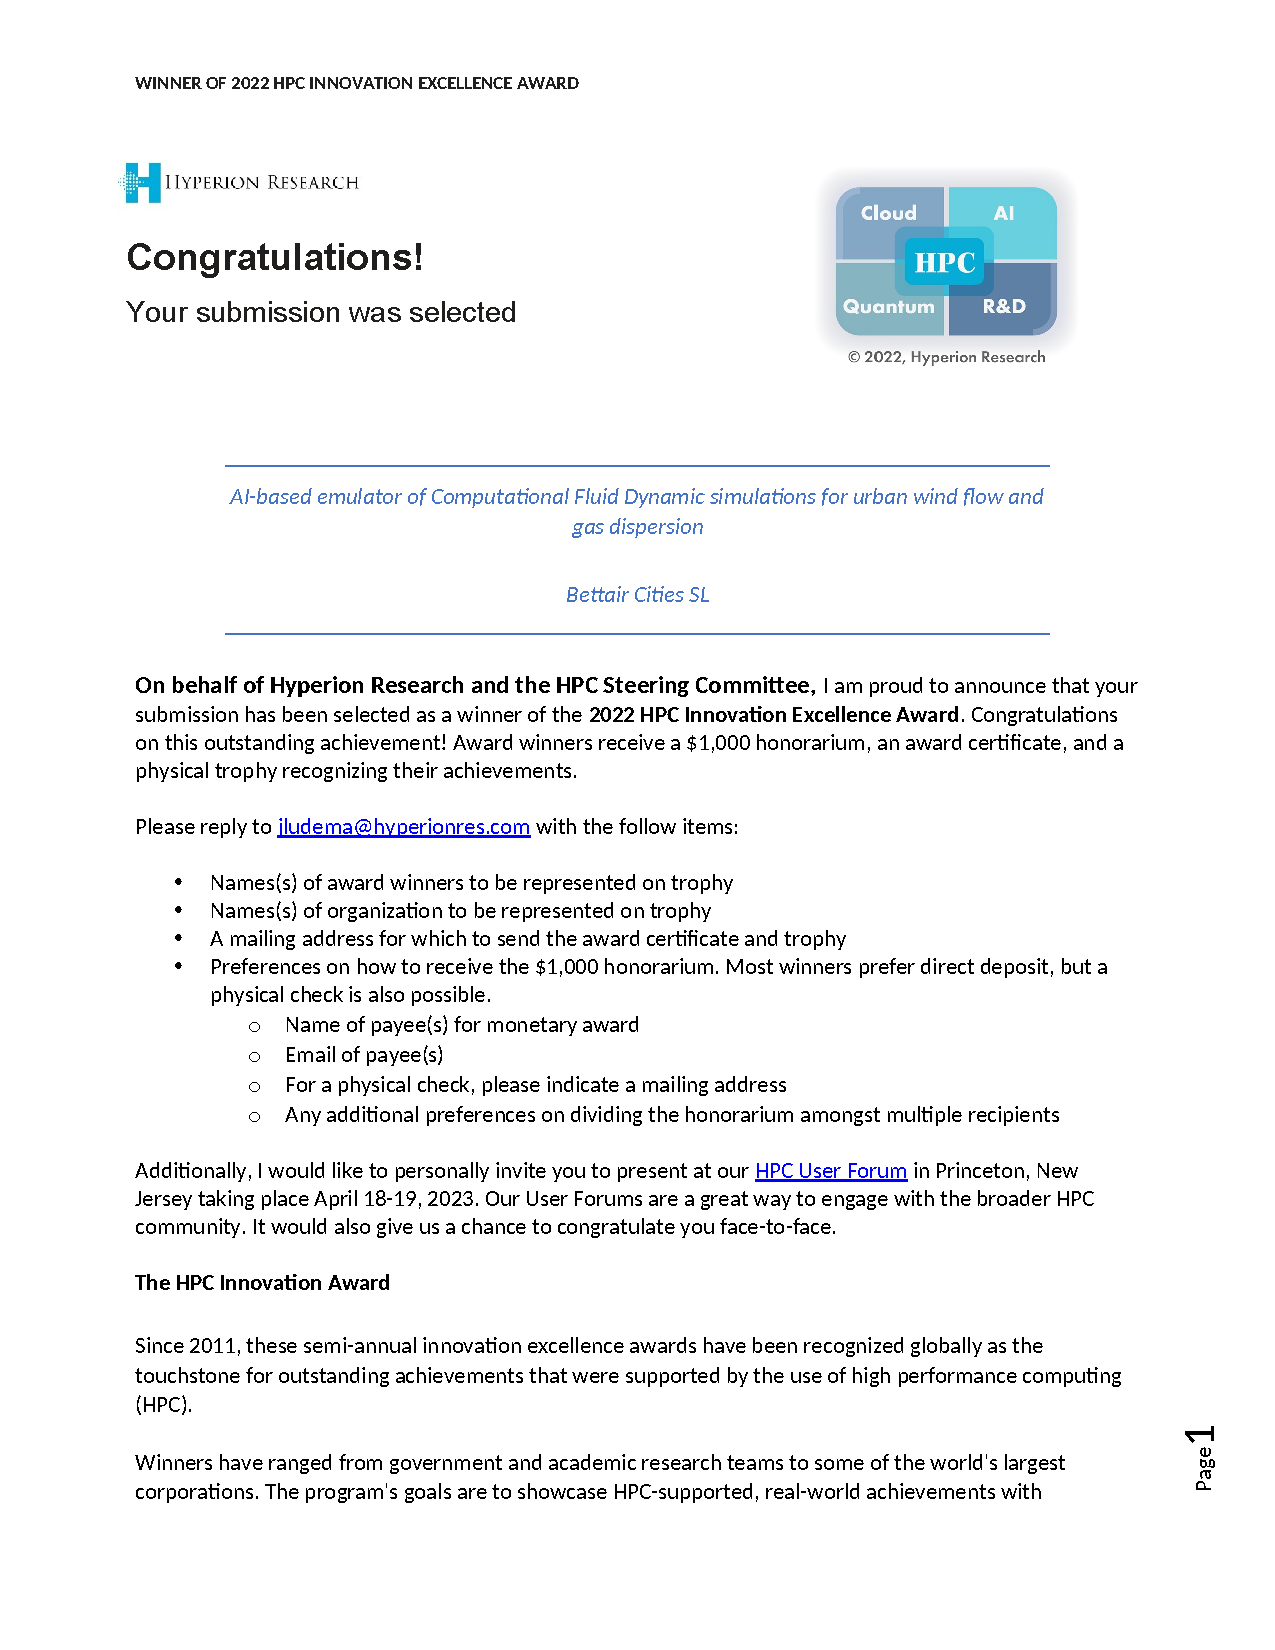
\includepdf[pages=-,link,linkname=hyperion-award,pagecommand={\refstepcounter{includepdfpage}\label{testing.\theincludepdfpage}}]{./documents_justificacio/2022-HPC-Innovation_Award.pdf}
\thispagestyle{empty}
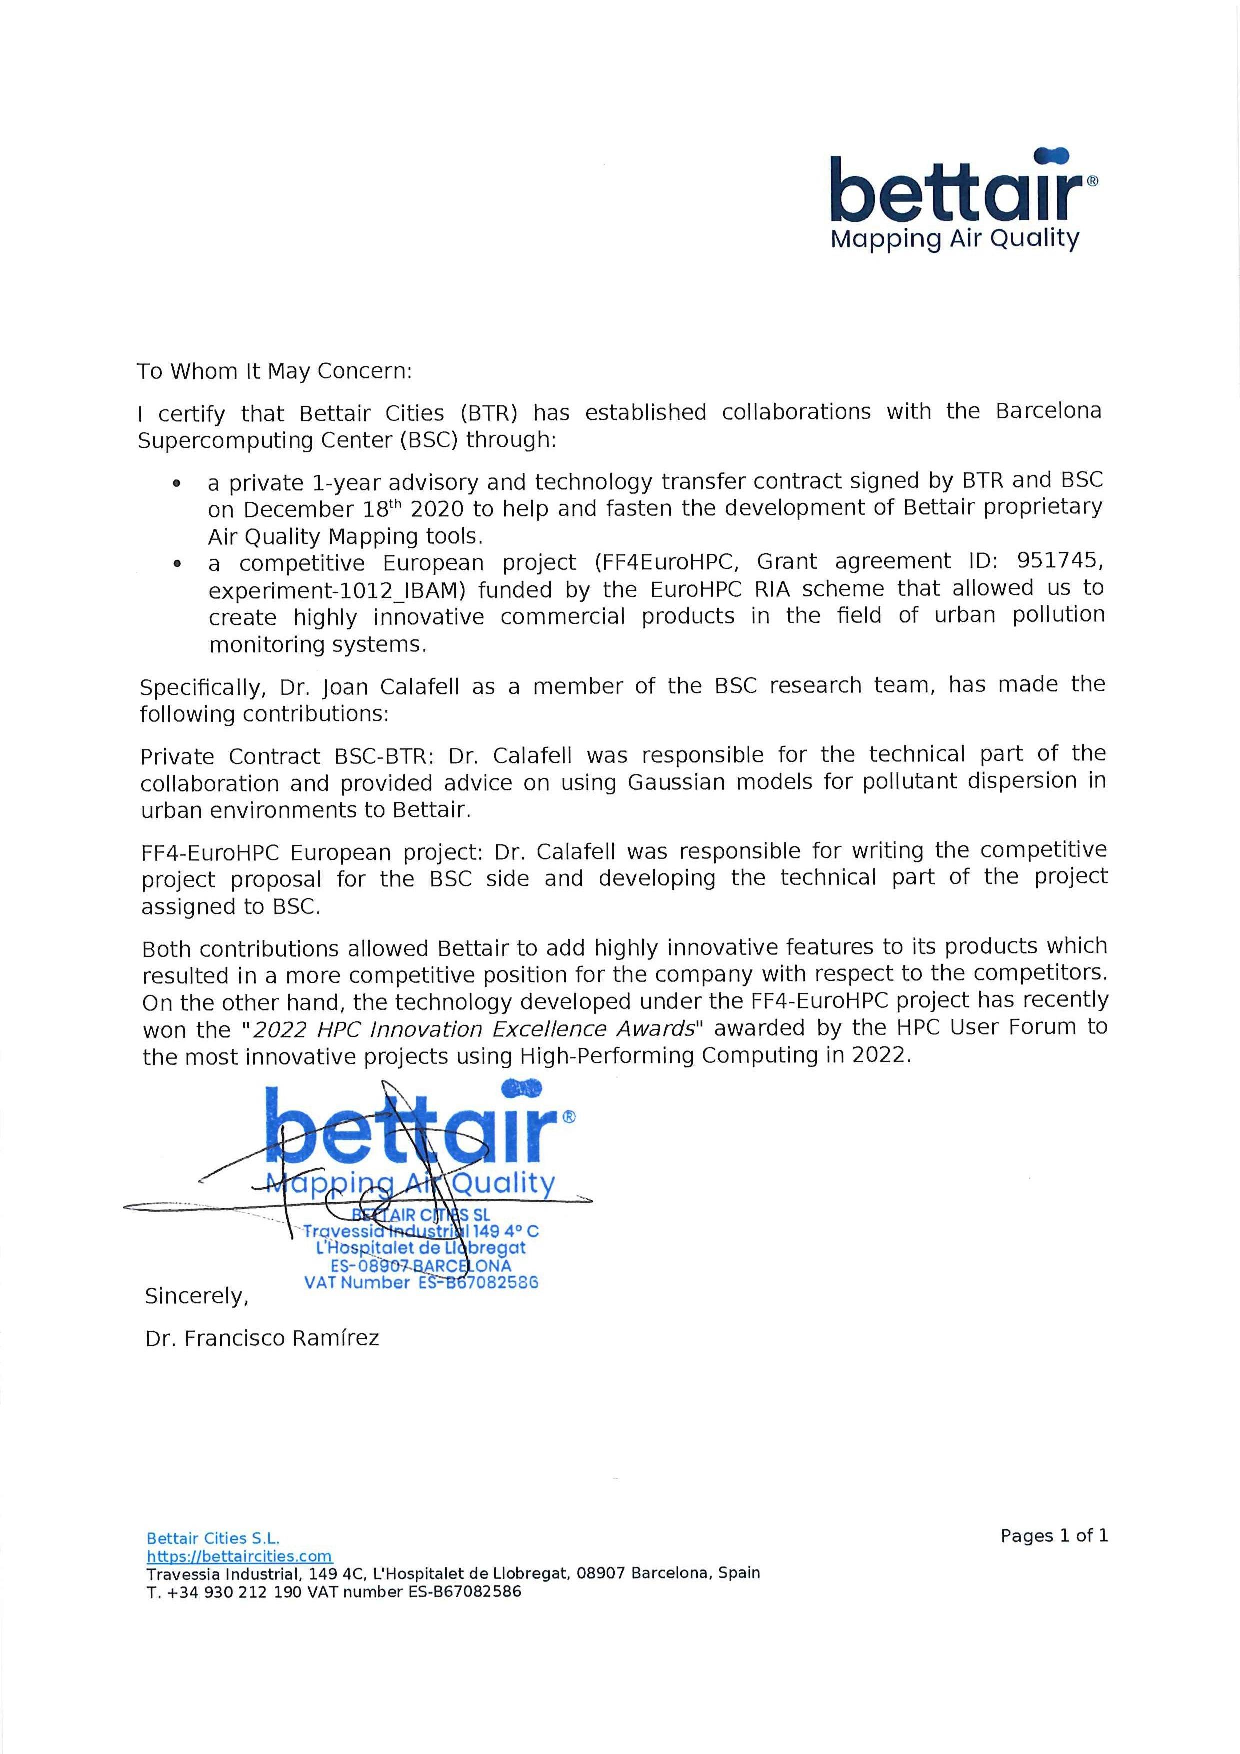
\includepdf[pages=-,link,linkname=carta-bettair,pagecommand={\refstepcounter{includepdfpage}\label{testing.\theincludepdfpage}}]{./documents_justificacio/Carta-Bettair.pdf}
\thispagestyle{empty}
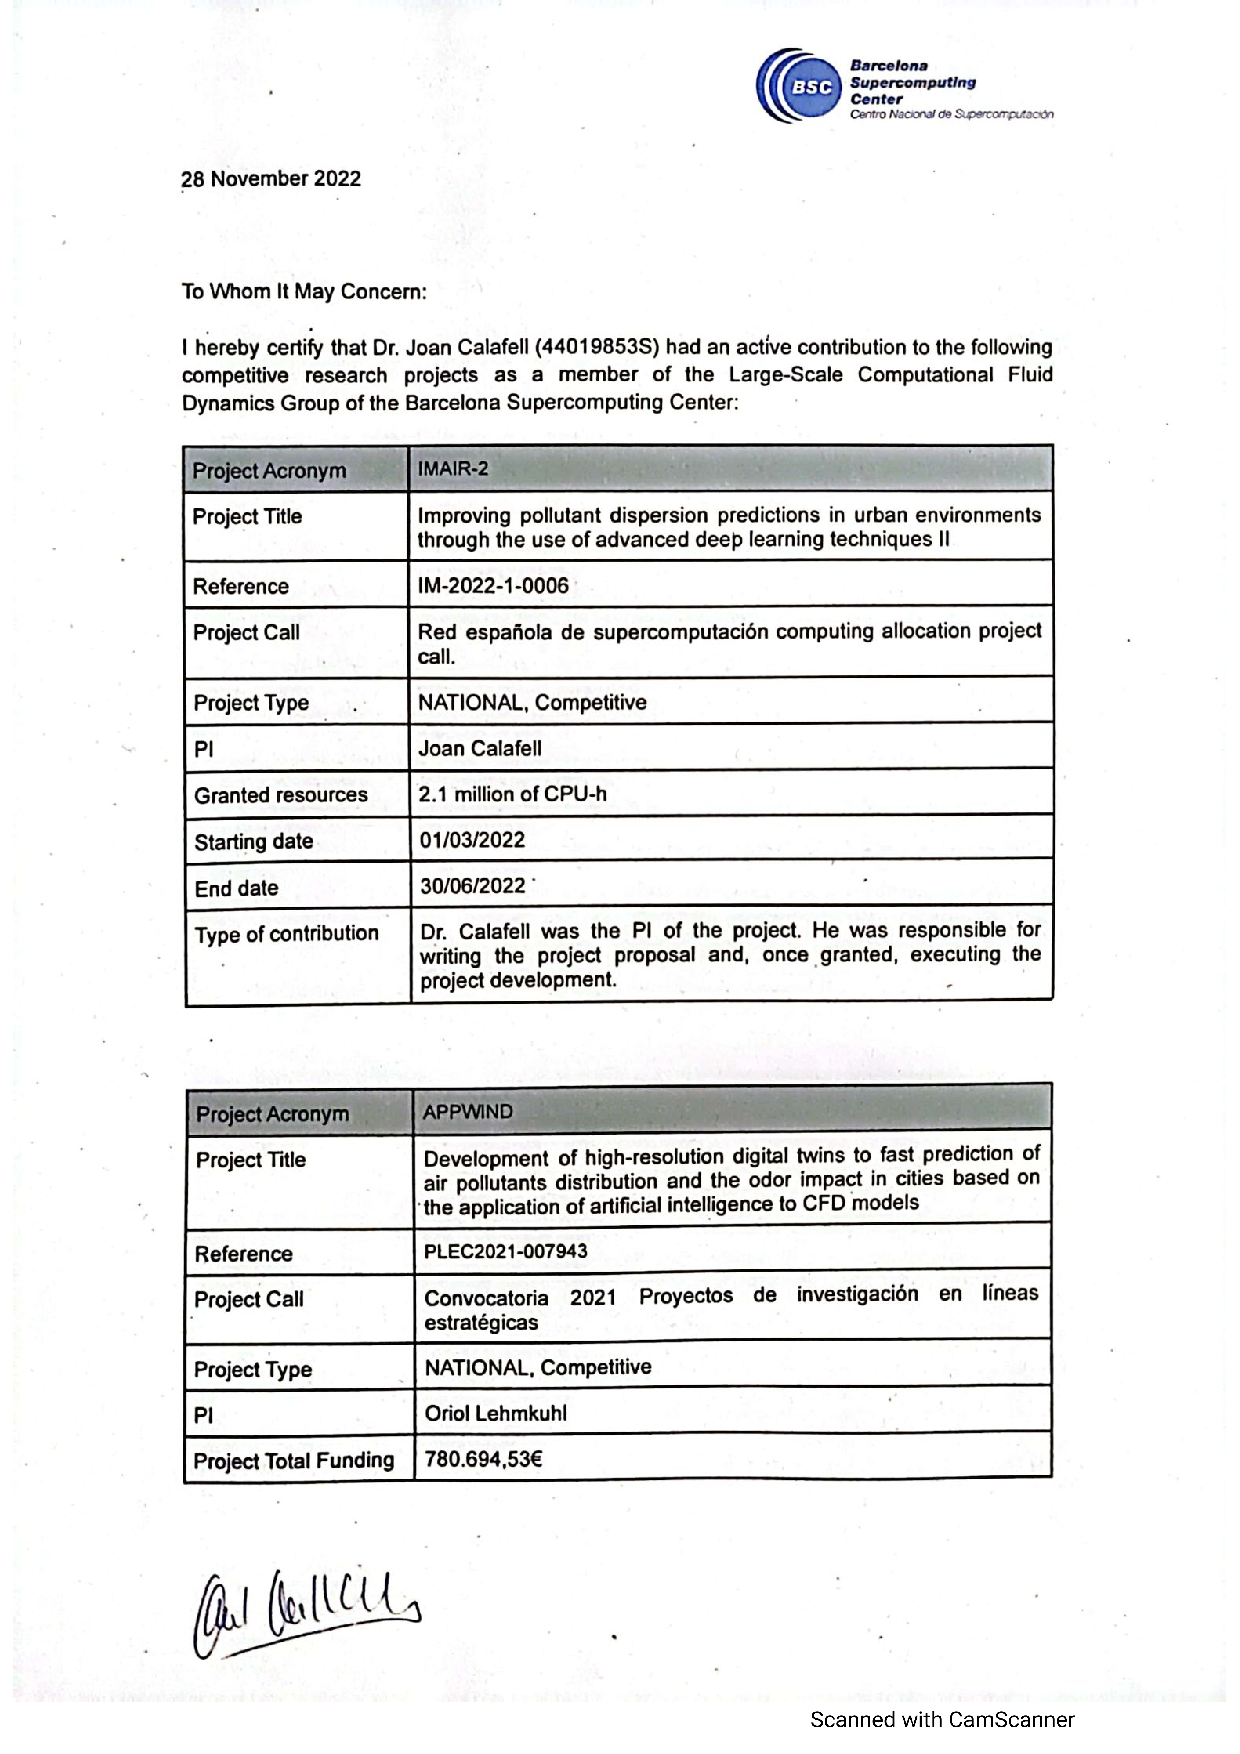
\includepdf[pages=-,link,linkname=projectes-bsc,pagecommand={\refstepcounter{includepdfpage}\label{testing.\theincludepdfpage}}]{./documents_justificacio/Projectes-BSC.pdf}
\thispagestyle{empty}
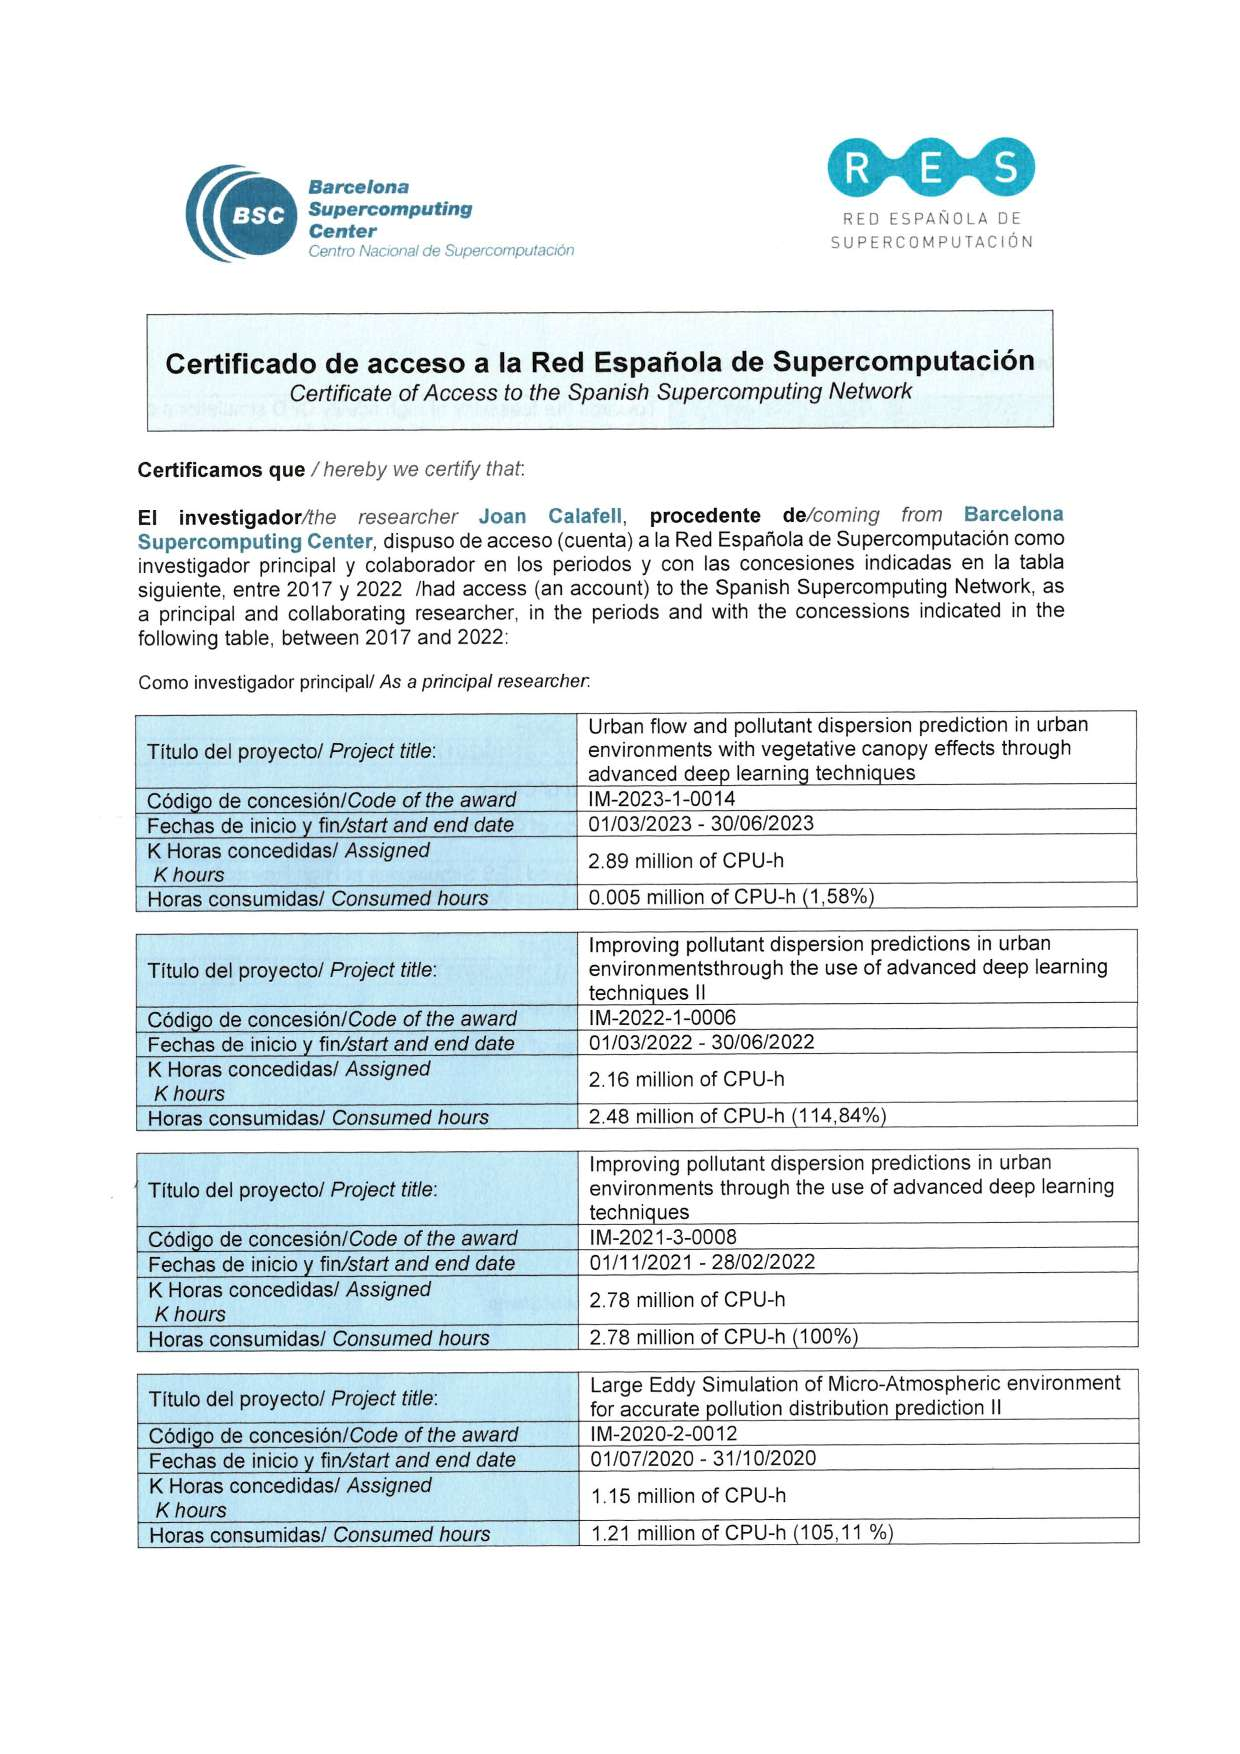
\includepdf[pages=-,link,linkname=projectes-res,pagecommand={\refstepcounter{includepdfpage}\label{testing.\theincludepdfpage}}]{./documents_justificacio/Projectes-RES.pdf}
\thispagestyle{empty}
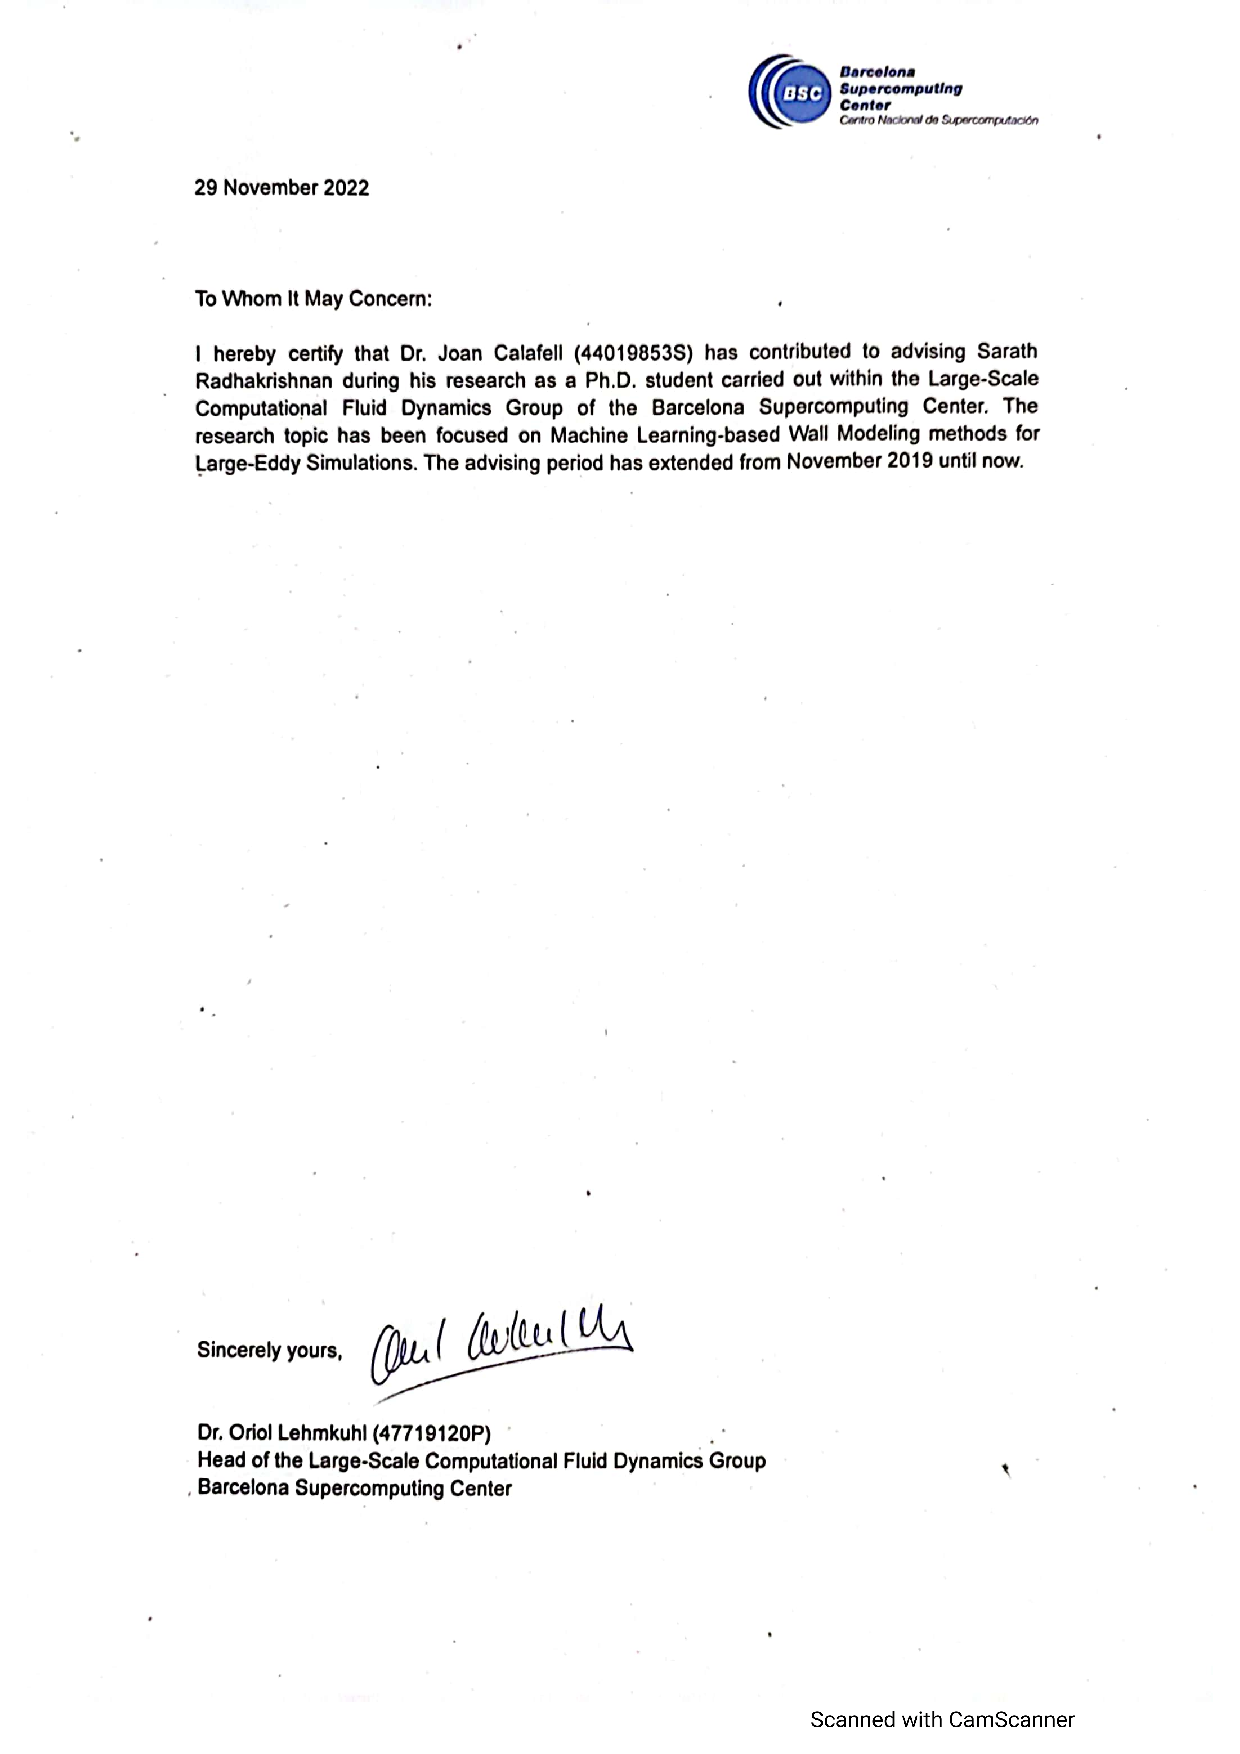
\includepdf[pages=-,link,linkname=tesis,pagecommand={\refstepcounter{includepdfpage}\label{testing.\theincludepdfpage}}]{./documents_justificacio/2022-Supervision-PhD.pdf}
\thispagestyle{empty}
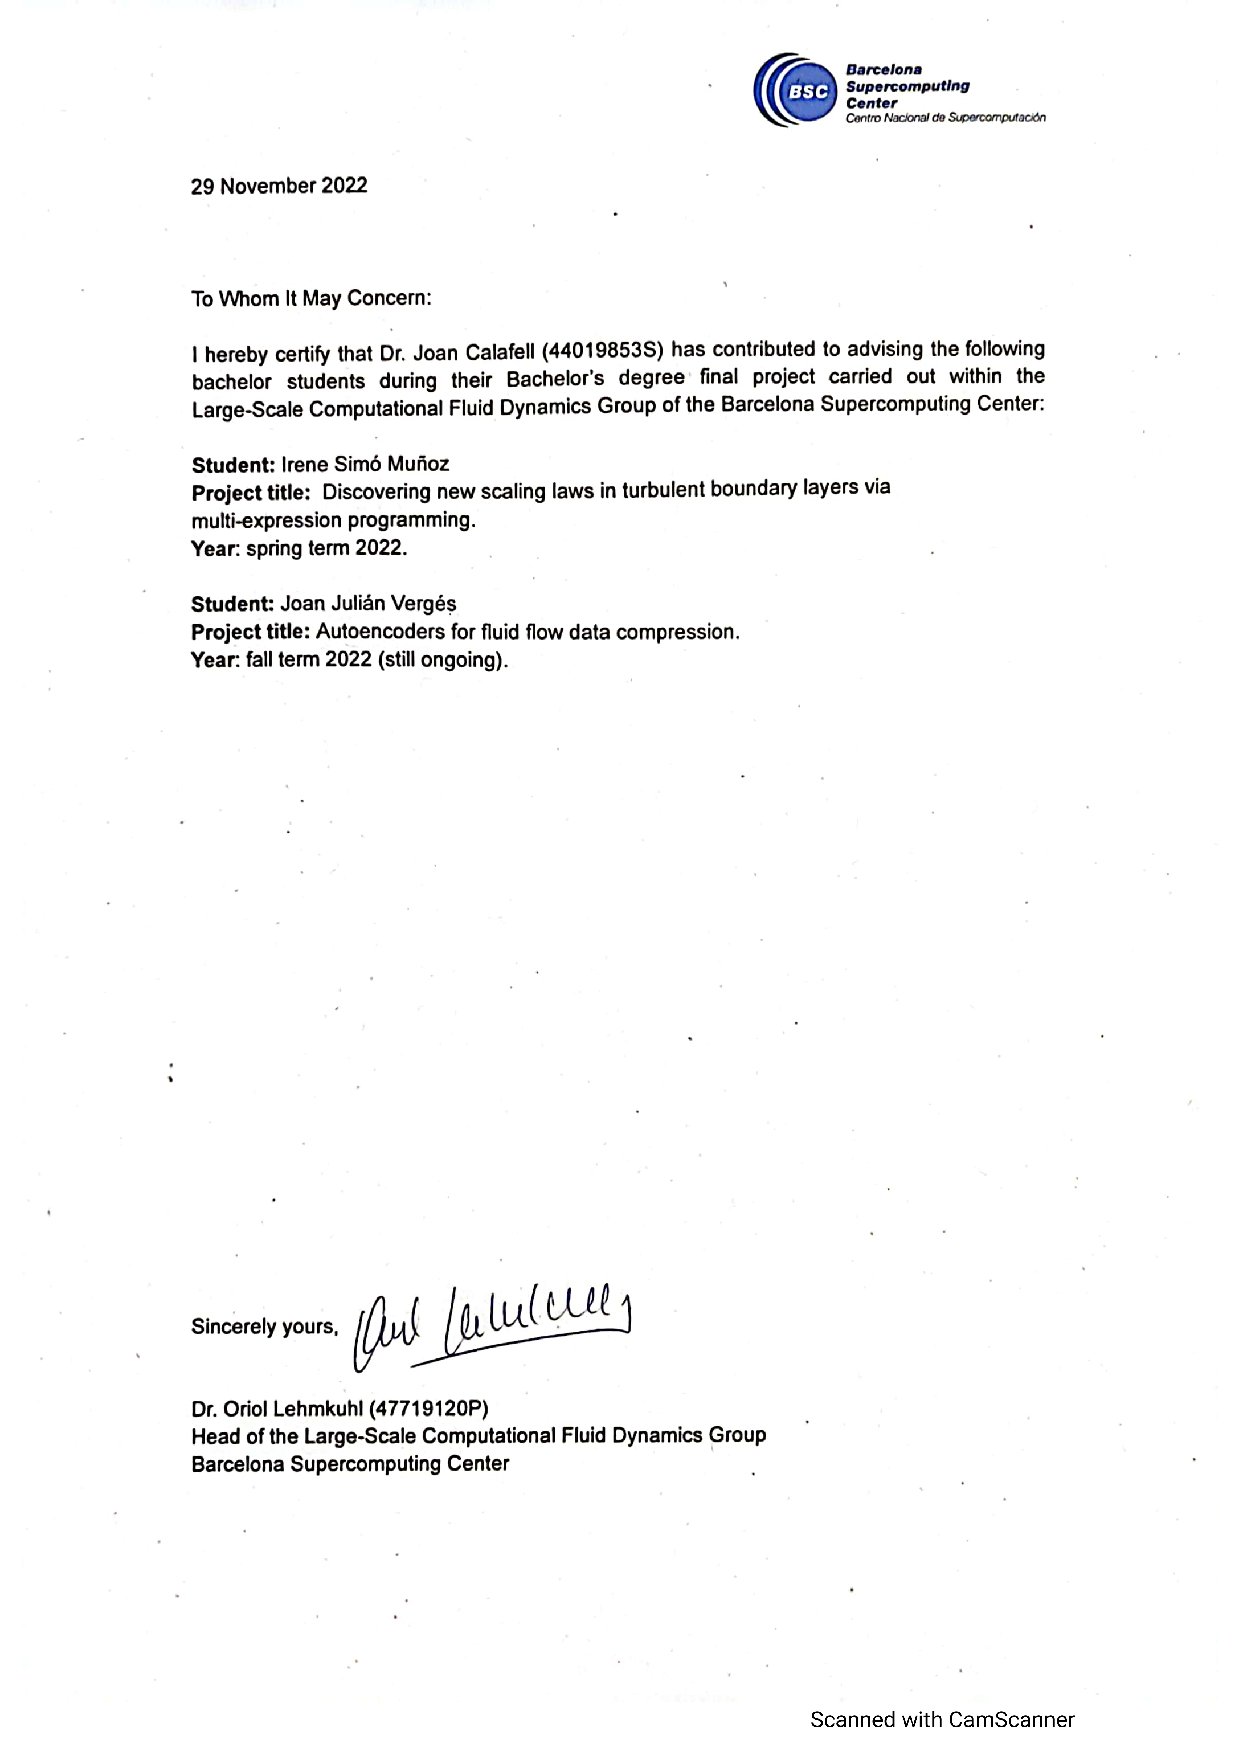
\includepdf[pages=-,link,linkname=tfg,pagecommand={\refstepcounter{includepdfpage}\label{testing.\theincludepdfpage}}]{./documents_justificacio/2022-Supervision-TFG.pdf}
\thispagestyle{empty}
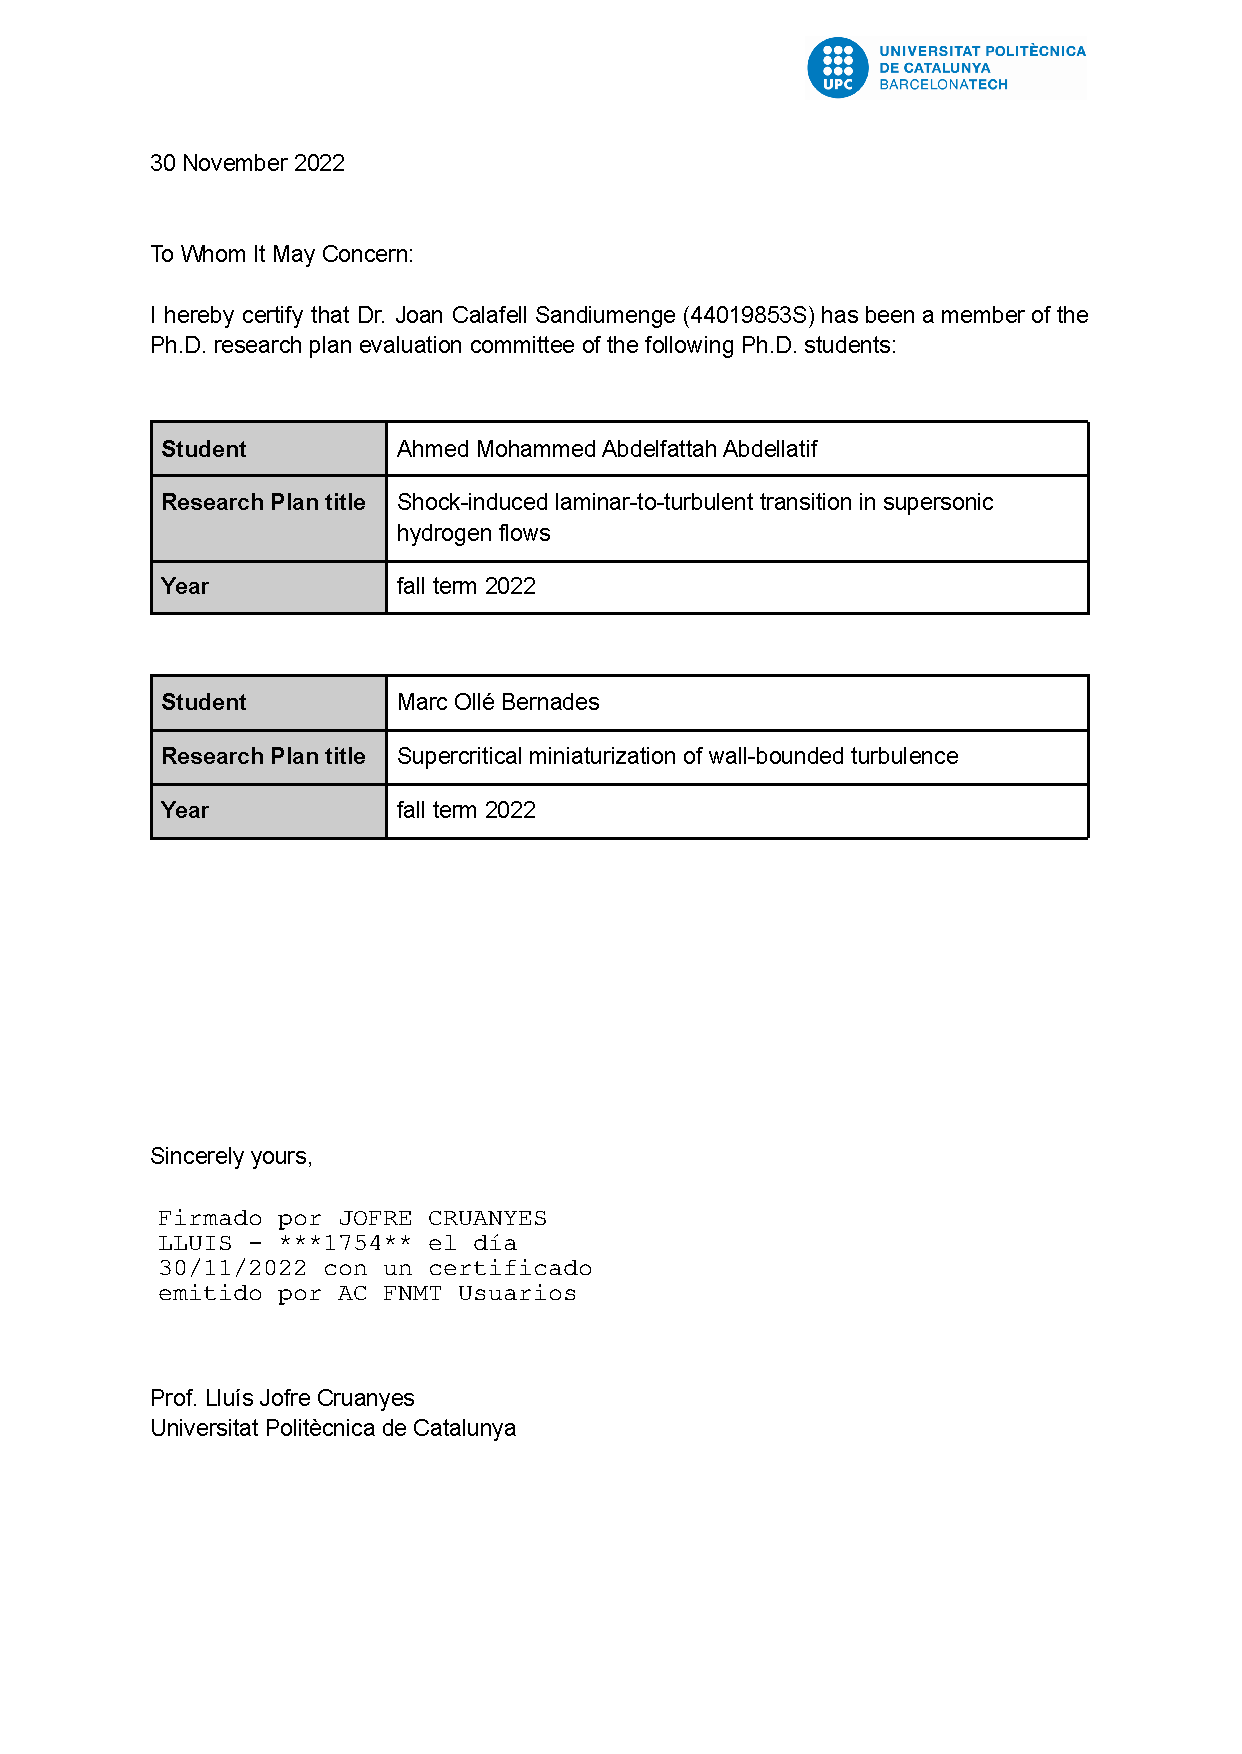
\includepdf[pages=-,link,linkname=tribunals,pagecommand={\refstepcounter{includepdfpage}\label{testing.\theincludepdfpage}}]{./documents_justificacio/2022-Tribunal-Research-Plan-UPC.pdf}
\thispagestyle{empty}
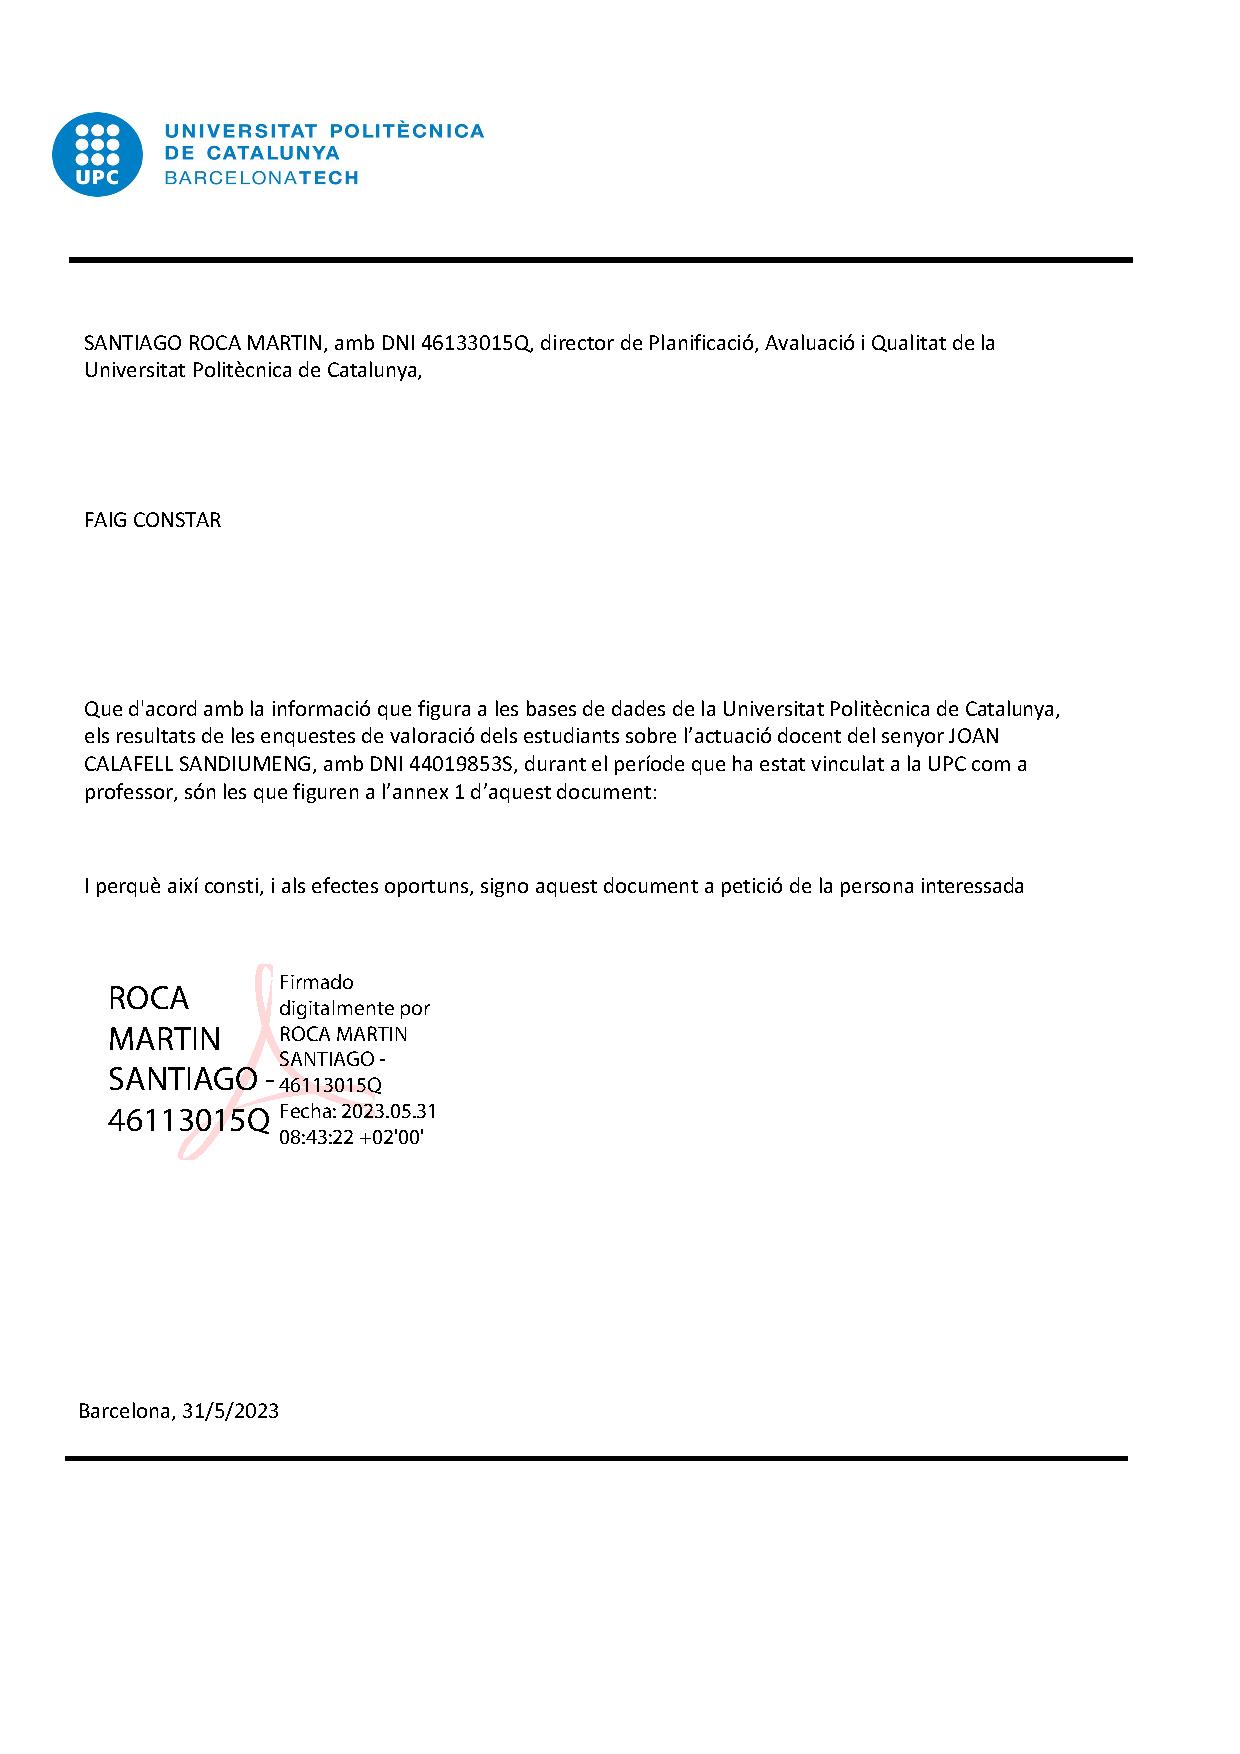
\includepdf[pages=-,link,linkname=enquestes,pagecommand={\refstepcounter{includepdfpage}\label{testing.\theincludepdfpage}}]{./documents_justificacio/Calafell-Enquestes.pdf}
\thispagestyle{empty}

\end{document}